\documentclass[a4paper, 12pt]{report}

\usepackage[dvipsnames]{xcolor}

%%%%%%%%%%%%%%%%
% Set Variables %
%%%%%%%%%%%%%%%%

\def\useItalian{0}  % 1 = Italian, 0 = English

\def\courseName{Mathematical Logic for Computer Science}

\def\coursePrerequisites{Sufficient knowledge of logic and theoretical computer science}

\def\book{\curlyquotes{Introduction to \\Mathematical Logic}, E. Mendelson}

\def\authorName{Simone Bianco}
\def\email{bianco.simone@outlook.it}
\def\github{https://github.com/Exyss/university-notes}
\def\linkedin{https://www.linkedin.com/in/simone-bianco}

%%%%%%%%%%%%
% Packages %
%%%%%%%%%%%%

\usepackage{../../packages/Nyx/nyx-packages}
\usepackage{../../packages/Nyx/nyx-styles}
\usepackage{../../packages/Nyx/nyx-frames}
\usepackage{../../packages/Nyx/nyx-macros}
\usepackage{../../packages/Nyx/nyx-title}
\usepackage{../../packages/Nyx/nyx-intro}

%%%%%%%%%%%%%%
% Title-page %
%%%%%%%%%%%%%%

\logo{../../packages/Nyx/logo.png}

\if\useItalian1
    \institute{\curlyquotes{\hspace{0.25mm}Sapienza} Università di Roma}
    \faculty{Ingegneria dell'Informazione,\\Informatica e Statistica}
    \department{Dipartimento di Informatica}
    \ifdefined\book
        \subtitle{Appunti integrati con il libro \book}
    \fi
    \author{\textit{Autore}\\\authorName}
\else
    \institute{\curlyquotes{\hspace{0.25mm}Sapienza} University of Rome}
    \faculty{Faculty of Information Engineering,\\Informatics and Statistics}
    \department{Department of Computer Science}
    \ifdefined\book
        \subtitle{Lecture notes integrated with the book \book}
    \fi
    \author{\textit{Author}\\\authorName}
\fi


\title{\courseName}
\date{\today}

% \supervisor{Linus \textsc{Torvalds}}
% \context{Well, I was bored\ldots}

%%%%%%%%%%%%
% Document %
%%%%%%%%%%%%

\addbibresource{./references.bib}

\begin{document}
    \maketitle

    % The following style changes are valid only inside this scope 
    {
        \hypersetup{allcolors=black}
        \fancypagestyle{plain}{%
        \fancyhead{}        % clear all header fields
        \fancyfoot{}        % clear all header fields
        \fancyfoot[C]{\thepage}
        \renewcommand{\headrulewidth}{0pt}
        \renewcommand{\footrulewidth}{0pt}}

        \romantableofcontents
    }

    \introduction

    %%%%%%%%%%%%%%%%%%%%%

    \chapter{Propositional logic}

    \section{Introduction to logical constructs}

    Logic is concerned with the validity of reasoning independently of the meaning of its components. In particular,\textbf{propositional logic} deals with studying the properties of certain logical constructs used in natural language as well as in scientific and mathematical practice. In particular, we're interested in the following constructs:
    \begin{itemize}
        \item \textit{Negation} (\( \neg \)): This operation inverts the truth value of a statement. If a statement is true, its negation is false, and vice versa.
        \item \textit{Conjunction} (\( \wedge \)): This operation represents the logical \curlyquotes{and}. The result is true if and only if both components are true.
        \item \textit{Disjunction} (\( \vee \)): This operation represents the logical \curlyquotes{or}. The result is true if at least one of the components is true.
        \item \textit{Implication} (\( \to \)): This operation represents the logical \curlyquotes{if \dots then} statement. The result is false only if the first component is true and the second component is false. In other words, this operator forces that when the premise holds, the conclusion must always follow (if the premise is false, we don't care about the truthfulness of the consequence).
        \item \textit{Equivalence} (\( \liff \)): This operation represents the logical \curlyquotes{if and only if} statement. The result is true when both components have the same truth value, i.e. they're either both true or both false.
    \end{itemize}
    
    For instance, consider the following simple arithmetic argument:
    \begin{enumerate}
        \item If \( a = 0 \) or \( b = 0 \), then \( a \cdot b = 0 \)
        \item \( a \cdot b \neq 0 \)
        \item \( a \neq 0 \) and \( b \neq 0 \)
    \end{enumerate}
    
    Intuitively, the third proposition \curlyquotes{follows} from the other two propositions, i.e. it is the conclusion of an argument with the first two as premises. To formalize this argument, we first identify those parts that cannot be further analyzed in terms of logical constructs and that can be true or false (called \textbf{atomic parts}). In our case, these atomic parts are \( a = 0 \), \( b = 0 \), and \( a \cdot b = 0 \).
    
    We assign a distinct letter to each of these atomic parts: for \( a = 0 \), we associate \( A \); for \( b = 0 \), we associate \( B \); and for \( a \cdot b = 0 \), we associate \( C \). Then, we replace the logical constructs in natural language (if \dots then, or, and, not) with formal symbols, called Boolean connectives: \( \neg \) for negation, \( \vee \) for disjunction, \( \wedge \) for conjunction, \( \rightarrow \) for implication (if \dots then), and \( \leftrightarrow \) for equivalence (if and only if). 
    
    We obtain the following formalization:
    \begin{enumerate}
        \item $(A \lor B) \to C$
        \item $\lnot C$
        \item $\lnot A \land \lnot B$
    \end{enumerate}

    where we read \( A \lor B \) as \curlyquotes{A or B}, \( \neg C \) as \curlyquotes{not C} and so on. Consider now the following verbal argument:
    \begin{enumerate}
        \item If the father is tall or the mother is tall, then the child is tall
        \item The child is short
        \item The father is short and the mother is short
    \end{enumerate}
    
    If we attempt a formalization of the argument, we quickly realize that we obtain the same formalization as the previous argument, where we write \( A \) for \curlyquotes{the father is tall}, \( B \) for \curlyquotes{the mother is tall}, and \( C \) for \curlyquotes{the child is tall}. Therefore, the two arguments are identical. Formal logic allows us to identify the common logical structure in arguments that deal with different objects and structures, as is the case in the examples above. However, in this case the first premise is obviously known to be empirically false. Nevertheless, if we assume it as premise for an argument, we intuitively recognize that the reasoning is \textbf{valid} (or correct). When we say the argument is valid (or correct), we mean that if the premises are true, then the conclusion is also true; \underline{not} that the premises are true.
    
    To evaluate the truthfulness of a propositional statement, we use \textbf{truth tables}. In logic, a truth table is a table used to determine whether a logical expression is true or false based on the \textbf{truth values} of its components. Truth tables are primarily used to evaluate the validity of logical propositions and determine the relationships between various logical statements. Each row of a truth table represents a unique combination of truth values for the variables involved in the logical expression. The columns show the intermediate truth values of the components of the expression, ultimately leading to the evaluation of the entire logical formula.

    \begin{figure}[H]
        \centering
        \begin{tabular}{c c c c c}
            \begin{tabular}{c|c}
                $A$ & $\lnot A$ \\
                \hline
                0 & 1 \\
                1 & 0
            \end{tabular}

            & \qquad \qquad &

            \begin{tabular}{cc|c}
                $A$ & $B$ & $A \land B$ \\
                \hline
                0 & 0 & 0 \\
                0 & 1 & 0 \\
                1 & 0 & 0 \\
                1 & 1 & 1 \\
            \end{tabular}

            & \qquad \qquad &

            \begin{tabular}{cc|c}
                $A$ & $B$ & $A \lor B$ \\
                \hline
                0 & 0 & 0 \\
                0 & 1 & 1 \\
                1 & 0 & 1 \\
                1 & 1 & 1 \\
            \end{tabular}
        \end{tabular}

        \vspace{15pt}

        \begin{tabular}{c c c}
            \begin{tabular}{cc|c}
                $A$ & $B$ & $A \to B$ \\
                \hline
                0 & 0 & 1 \\
                0 & 1 & 1 \\
                1 & 0 & 0 \\
                1 & 1 & 1 \\
            \end{tabular}

            & \qquad \qquad &

            \begin{tabular}{cc|c}
                $A$ & $B$ & $A \liff B$ \\
                \hline
                0 & 0 & 1 \\
                0 & 1 & 0 \\
                1 & 0 & 0 \\
                1 & 1 & 1 \\
            \end{tabular}
        \end{tabular}

        \caption{Truth tables of the five logical operators previously introduces. The value 0 represents the falseness of the propositions, while the value 1 represents their truthfulness.}
    \end{figure}

    Consider now a more complex logical expression \( A \rightarrow (B \wedge C) \). A truth table for this expression requires evaluating the truth values for \( A \), \( B \) and \( C \), then determining the truth value of the conjunction \( B \wedge C \), and finally computing the implication \( A \rightarrow (B \wedge C) \).

    \begin{figure}[H]
        \centering
        
        \begin{tabular}{ccc|c|c}
            \( A \) & \( B \) & \( C \) & \( B \wedge C \) & \( A \rightarrow (B \wedge C) \) \\
            \hline
            0 & 0 & 0 & 0 & 1 \\
            0 & 0 & 1 & 0 & 1 \\
            0 & 1 & 0 & 0 & 1 \\
            0 & 1 & 1 & 1 & 1 \\
            1 & 0 & 0 & 0 & 0 \\
            1 & 0 & 1 & 0 & 0 \\
            1 & 1 & 0 & 0 & 0 \\
            1 & 1 & 1 & 1 & 1 \\
        \end{tabular}

        \label{form_1}
        \caption{Truth table for the logical expression  \( A \rightarrow (B \wedge C) \)}
    \end{figure}

    \section{Mathematical formalization}

    The first step is to define a completely rigorous formal language that can be subjected to mathematical study. For propositional logic, the procedure is simple: propositions are formalized by formulas obtained by applying Boolean connectives to some atomic building blocks, called \textit{propositional variables}. These variables intuitively represent propositions that cannot be further analyzed in terms of logical operators such as negation, conjunction, disjunction, implication, or equivalence.

    \begin{frameddefn}{Language and propositions}
        A propositional language is a set $\mathcal{L} = \{p_1, \ldots, p_n\}$, where each $p_i$ is a symbol called propositional variable. Given a propositional language $\mathcal{L}$, the set of propositions (or valid formulas) over $\mathcal{L}$, denoted with $\mathsf{PROP}_\mathcal{L}$ (or $\mathsf{FML}_\mathcal{L}$), is the minimal set of \underline{finite} expressions over $\mathcal{L} \cup \{\lnot, \land, \lor, \to, \liff\}$ such that: 
        \begin{itemize}
            \item Each propositional variable in $\mathcal{L}$ is a proposition, i.e. $\mathcal{L} \subseteq \mathsf{PROP}_\mathcal{L}$
            \item If $A \in \mathsf{PROP}_\mathcal{L}$ then $\lnot A \in \mathsf{PROP}_\mathcal{L}$
            \item If $A,B \in \mathsf{PROP}_\mathcal{L}$ then $(A \land B), (A \lor B), (A \to B), (A \liff B) \in \mathsf{PROP}_\mathcal{L}$
        \end{itemize}
    \end{frameddefn}

    When $\mathcal{L}$ is non-ambiguous in the context, we denote $\mathsf{PROP}_\mathcal{L}$ directly as $\mathsf{PROP}$. Moreover, to make expressions easier to read, we use the following precedence rules: $\lnot$ has precedence over $\land, \lor$, while $\land, \lor$ have precedence over $\to, \liff$. In other words, we have that $(\lnot((\lnot A) \lor B)) \to C$ can be written as $\lnot(\lnot A \lor B) \to C$.

    After formalizing the concept of propositional language and propositions, we're ready to formalize the concept of truth tables. Each row of a truth table can be described through \textbf{assignments}. Here, an assignment is any function $\alpha : \mathcal{L} \to \{0,1\}$, i.e. a map that assigns a truth value to each propositional variable of the language. By extension, any assignment over $\mathcal{L}$ induces an assignment over $\mathsf{PROP}$. These assignments are functions $\widehat{\alpha} : \mathsf{PROP} \to \{0,1\}$ inductively defined as:
    \[\widehat{\alpha}(A) = \alpha(A) \text{ when } A \in \mathcal{L}\]
    \[\widehat{\alpha}(\lnot A) = \soe{ll}{
        1 & \text{if } \widehat{\alpha}(A) = 0 \\
        0 & \text{if } \widehat{\alpha}(A) = 1 \\
    }\]

    \[\widehat{\alpha}(A \land B) = \soe{ll}{
        1 & \text{if } \widehat{\alpha}(A) = \widehat{\alpha}(B) = 1 \\
        0 & \text{otherwise} \\
    }\]

    \[\widehat{\alpha}(A \lor B) = \soe{ll}{
        0 & \text{if } \widehat{\alpha}(A) = \widehat{\alpha}(B) = 0 \\
        1 & \text{otherwise} \\
    }\]

    \[\widehat{\alpha}(A \to B) = \soe{ll}{
        0 & \text{if } \widehat{\alpha}(A) = 1 \text{ and } \widehat{\alpha}(B) = 0 \\
        1 & \text{otherwise} \\
    }\]

    \[\widehat{\alpha}(A \liff B) = \soe{ll}{
        1 & \text{if } \widehat{\alpha}(A) = \widehat{\alpha}(B) \\
        0 & \text{otherwise} \\
    }\]

    To make notation easier, we'll directly refer to $\widehat{\alpha}$ as $\alpha$. Using the concept of assignments, we can also define the concept of \textbf{logical equivalence}. Informally, two formulas are said to be logically equivalent when they share the same exact truth table.
    
    \begin{frameddefn}{Logical equivalence}
        We say that two formulas $A, B \in \mathsf{PROP}$ are logically equivalent, denoted with $A \equiv B$, when for every assignment $\alpha$ it holds that $\alpha(A) = \alpha B$.
    \end{frameddefn}

    By definition, it clearly holds that $\equiv$ is an equivalence relation since it is reflexive, symmetric and transitive. Logical equivalences allow us to treat logical components as if they were algebraic operators. For instance, common algebraic properties include:
    \begin{itemize}
        \item \textit{Involution}: $\lnot \lnot A \equiv A$
        \item \textit{Idempotency}: $A \lor A \equiv A$ and $A \land A \equiv A$
        \item \textit{Associativity}: $(A \lor B) \lor C \equiv A \lor (B \lor C)$ and $(A \land B) \land C \equiv A \land (B \land C)$
        \item \textit{Commutativity}: $A \lor B \equiv B \lor A$ and $A \land B \equiv B \land A$
        \item \textit{Distributivity}:  $A \lor (B \land C) \equiv (A \lor B) \land (A \lor C)$ and $A \land (B \lor C) \equiv (A \land B) \lor (A \land C)$
        \item \textit{De Morgan's law}: $\lnot(A \lor B) \equiv \lnot A \land \lnot B$ and $\lnot(A \land B) \equiv \lnot A \lor \lnot B$
    \end{itemize}

    Through these basic properties, we notice that each connective can be rewritten in terms of the other connectives. In fact, we could define propositional logic using only $\lnot$ and $\land$ (or $\lnot$ and $\lor$). This property is very useful in circuit logic.
    \begin{itemize}
        \item $A \land B \equiv \lnot(\lnot A \lor \lnot B)$
        \item $A \lor B \equiv \lnot(\lnot A \land \lnot B)$
        \item $A \to B \equiv \lnot A \lor B$
        \item $A \liff B \equiv (A \to B) \land (B \to A)$
    \end{itemize}

    If for an assignment $\alpha$ and a formula $A$ it holds that $\alpha(A) = 1$, we say that $\alpha$ \textit{satisfies} $A$. If $A$ has at least one satisfying assignment, we say that $A$ is \textbf{satisfiable}. When no satisfying assignment exists, we say that the formula $A$ is \textbf{unsatisfiable}. On the contrary, when every possible assignment satisfies $A$ we say that $A$ is a \textbf{tautology} (or \textit{logical truth}, \textit{logically valid}). By definition, tautologies represent statements that are always true, no matter the situation. We denote with $\mathsf{SAT}, \mathsf{UNSAT}$ and $\mathsf{TAUT}$ the sets of satisfiable, unsatisfiable and tautological formulas. By definition, we have that $F \in \mathsf{TAUT}$ if and only if $\lnot F \in \mathsf{UNSAT}$.
    If a formula is not a tautology, we cannot ensure the truthfulness of the statement. Hence, we consider \textit{true statements} only as formulas that are \textit{always true} (the set $\mathsf{TAUT}$), while we consider \textit{false statement} as formulas that are \textit{not always true} (the set $\mathsf{UNSAT} \cup (\mathsf{SAT} - \mathsf{TAUT})$). 
    
    With a slight abuse of notation, we define $1$ and $0$ as the formulas such that for every assignment it holds that $\alpha(1) = 1$ and $\alpha(0) = 0$. This allows us to further simplify logical equivalences algebraically:
    \begin{itemize}
        \item \textit{Absorption law}: $A \lor 0 \equiv A$ and $A \land 1 \equiv A$
        \item \textit{Cancellation law}: $A \lor 1 \equiv 1$ and $A \land 0 \equiv 0$
        \item \textit{Tertium non datur}: $A \lor \lnot A \equiv 1$ and $A \land \lnot A \equiv 0$
    \end{itemize}

    Using all the algebraic rules that we have shown, we can easily evaluate propositional formulas by first reducing them to a smaller equivalent formula and then (eventually) by evaluating the truth table of the reduced form:
    \[\begin{split}
        A \lor B \to B \lor \lnot C &\equiv \lnot (A \lor B) \lor B \lor \lnot C \\
        & \equiv (\lnot A \land \lnot B) \lor B \lor \lnot C \\
        & \equiv ((\lnot A \lor B) \land (\lnot B \lor B)) \lor \lnot C \\
        & \equiv ((\lnot A \lor B) \land 1) \lor \lnot C \\
        & \equiv \lnot A \lor B \lor \lnot C \\
    \end{split}\]

    The concepts of tautology and unsatisfiability are strictly related with the concept of \textbf{logical consequence} that we have discussed in the previous section.

    \begin{frameddefn}{Logical consequence}
        Given the formulas $A_1, \ldots, A_n, A$, we say that $A$ is a logical consequence of $A_1, \ldots, A_n$, written as $A_1, \ldots, A_n \models A$ if whenever $A_1, \ldots, A_n$ are true $A$ is also true.
    \end{frameddefn}

    Through truth tables, evaluating if we can conclude $A$ through $A_1, \ldots, A_n$ is pretty easy: $A_1, \ldots, A_n \models A$ if and only if for every row where $A_1, \ldots, A_n$ are evaluated as 1 we also have that $A$ is evaluated as 1. For instance consider the \textit{Logician party} problem, made of the following propositions:
    \begin{enumerate}
        \item If the Logician party wins the elections then the taxes will increase if the deficit remains high
        \item If the Logician party wins the elections, the deficit remains high
        \item If the Logician party wins the elections, the taxes will increase
    \end{enumerate}
    
    We want to know if the last proposition is a logical consequence of the other two propositions. First, we define the following propositional variables:
    \begin{itemize}
        \item Let $P$ be the variable such that $P = 1$ if and only if the Logician party wins the elections
        \item Let $T$ be the variable such that $T = 1$ if and only if the taxes will increase
        \item Let $D$ be the variable such that $D = 1$ if and only if the deficit remains high
    \end{itemize}

    Using the three variables, we formalize the three propositions as follows:
    \begin{enumerate}
        \item $P \to (D \to T) \equiv \lnot P \lor (\lnot D \lor T) \equiv \lnot P \lnot D \lor T$ 
        \item $P \to D \equiv \lnot P \lor D$
        \item $P \to T \equiv \lnot P \lor D$
    \end{enumerate}

    \newpage

    Then, we compute the truth table for the problem:
    \begin{figure}[H]
        \centering
        
        \begin{tabular}{ccc|cc|c}
            $P$ & $T$ & $D$ & $\lnot P \lnot D \lor T$ & $\lnot P \lor D$ & $\lnot P \lor T$ \\
            \hline
            0 & 0 & 0 & 1 & 1 & 1 \\
            0 & 0 & 1 & 1 & 1 & 1 \\
            0 & 1 & 0 & 1 & 1 & 1 \\
            0 & 1 & 1 & 1 & 1 & 1 \\
            1 & 0 & 0 & 1 & 0 & 0 \\
            1 & 0 & 1 & 1 & 0 & 1 \\
            1 & 1 & 0 & 0 & 1 & 0\\
            1 & 1 & 1 & 1 & 1 & 1\\
         \end{tabular}

        \label{form_1}
        \caption{Truth table for the Logician party problem.}
    \end{figure}

    We observe that for every assignment $\alpha$ such that $\alpha(P \to (D \to T)) = 1$ and $\alpha(P \to D) = 1$, it also holds that $\alpha(P \to T) = 1$. Hence, we can indeed conclude that $P \to (D \to T), P \to D \models P \to T$. Since the number of rows in a truth table is exponential with respect to the number of propositional variables, enumerating the whole truth table may be too expensive. For instance, with only $4$ variables we would have to enumerate $2^4 = 16$ rows. To help with this issue, the following theorem comes in handy.

    \begin{framedthm}{}
        Given the formulas $A_1, \ldots, A_n, A$, the three following statements are equivalent:
        \begin{enumerate}
            \item  $A_1, \ldots, A_n \models A$
            \item  $(A_1 \land \ldots \land A_n \to A) \in \mathsf{TAUT}$
            \item  $(A_1 \land \ldots \land A_n \land \lnot A) \in \mathsf{UNSAT}$
        \end{enumerate}
    \end{framedthm}

    \begin{proof} Omitted (trivial) \end{proof}

    Hence, in order to evaluate if $A_1, \ldots, A_n \models A$ holds, we can show that $(A_1 \land \ldots \land A_n \to A) \equiv 1$ or that $(A_1 \land \ldots \land A_n \land \lnot A) \equiv 0$ through the algebraic properties shown before.
    
    For instance, consider the \textit{self-destruction button} problem. We must travel far away into the galaxy and Adam lends us his spaceship. Adams tells us that the spaceship has three buttons and that one and only one of them triggers the self-destruction protocol, while the others do nothing. Moreover, each of the three buttons has a post-it attached to it. The first and second button say \curlyquotes{I'm not the self-destruction button}, while the third button says \curlyquotes{The first button is the self-destruction button}. Adam tells us that one and only one of the buttons says the truth. Using pure logic, we have to find out which button is the self-destruction one in order to avoid blowing up ourselves.
    
    First, we define three propositional variables:
    \begin{itemize}
        \item Let $A$ be the variable such that $A = 1$ if and only if the first button triggers the self-destruction protocol
        \item Let $B$ be the variable such that $B = 1$ if and only if the second button triggers the self-destruction protocol
        \item Let $C$ be the variable such that $C = 1$ if and only if the third button triggers the self-destruction protocol
    \end{itemize}

    Then, we formalize the entire problem through the following two propositions $\phi, \psi$:
    \begin{enumerate}
        \item One and only one of the buttons triggers the self-destruction protocol, i.e.
        \[\phi = (A \lor B \lor C) \land \lnot (A \land B) \land \lnot (A \land C) \land \lnot (B \land C) \]
        \item One and only one of the buttons says the truth, i.e.
        \[\psi = (\lnot A \lor \lnot B \lor A) \land \lnot (\lnot A \land \lnot B) \land \lnot (\lnot A \land A) \land \lnot (\lnot B \land A) \]
    \end{enumerate}
    
    We observe that $\phi$ cannot be reduced too much: 
    \[\begin{split}
        \phi &= (A \lor B \lor C) \land \lnot (A \land B) \land \lnot (A \land C) \land \lnot (B \land C) \\
        &\equiv (A \lor B \lor C) \land (\lnot A \lor \lnot B) \land (\lnot A \lor \lnot C) \land (\lnot B \lor \lnot C)
    \end{split}\]

    However, $\psi$ can be reduced completely:
    \[\begin{split}
        \psi &= (\lnot A \lor \lnot B \lor A) \land \lnot (\lnot A \land \lnot B) \land \lnot (\lnot A \land A) \land \lnot (\lnot B \land A) \\
        &\equiv 1 \land \lnot (\lnot A \land \lnot B) \land \lnot 0 \land \lnot (\lnot B \land A) \\
        &\equiv (A \lor B) \land (B \lor \lnot A) \\
        &\equiv B
    \end{split}\]

    Thus, it's very easy to see that $\phi \land \psi \to B$ is indeed a tautology:
    \[\begin{split}
        \phi \land \psi \to B & \equiv \lnot(\phi \land \psi) \lor B \\
        &\equiv \lnot \phi \lor \lnot \psi \lor B \\
        &\equiv \lnot \phi \lor \lnot B \lor B \\
        &\equiv 1
    \end{split} \]

    Hence, this concludes that $\phi, \psi \models B$ and thus that the second button is the self-destruction one. However, we still observe that this alternative procedure may be as tedious as enumerating the whole truth table, even though it is usually faster. Currently, \underline{there are no} \underline{efficient procedures} that can answer questions such as \curlyquotes{is $F$ satisfiable?}, \curlyquotes{is $F$ unsatisfiable?} and \curlyquotes{is $F$ a tautology?}. Finding such algorithm or proving that such algorithm cannot exist is equivalent to solving the Millennium Problem $\mathsf{P} \stackrel{?}{=} \mathsf{NP}$, which asks the question \curlyquotes{can every efficiently verifiable problem also be efficiently solved?}. For this problem, the \textit{Clay Mathematical Institute} offers a prize of one million dollars. In many cases, it is possible to decide whether a certain proposition is a tautology or not, or whether a certain conclusion is a logical consequence of other propositions without constructing the truth table, but only by reasoning rigorously at a higher level.

    \section{Disjunctive and Conjunctive Normal Forms}

    Every propositional formula can be rewritten in a standard way. In particular, we have two standard ways to write a formula: the \textbf{Disjuntive Normal Form (DNF)} and the \textbf{Conjunctive Normal Form (CNF)}. A formula is said to be in DNF if it is a disjuction of AND clauses. An AND \textit{clause} is a conjunction of literals. A \textit{literal} is a propositional variable or a negation of a propositional variable. In other words, we say that $F$ is in DNF if:
    \[F = \bigvee_{j = 1}^m D_j = \bigvee_{j = 1}^m (\ell_{1, j} \land \ell_{2, j} \land \ldots \land \ell_{k_j, j})\]
    where each $D_j$ is an AND clause of the formula and each $\ell_{i_h}$ is a literal. Similarly, a formula is said to be in CNF if it is a conjunction of OR clauses.
    \[F = \bigwedge_{j = 1}^m C_j = \bigwedge_{j = 1}^m (\ell_{1, j} \lor \ell_{2, j} \lor \ldots \lor \ell_{k_j, j})\]

    Using the logical equivalence properties, it's clear that every formula has an equivalent DNF and CNF formula. In a more direct way, we can use truth tables (hence assignments) to yield an equivalent DNF or CNF formula.
    
    \begin{framedthm}{Equivalent DNF and CNF formulas}
        For every formula $F$ there is a DNF formula $F^{\mathsf{DNF}}$ and a CNF formula $F^{\mathsf{CNF}}$ such that $F \equiv F^{\mathsf{DNF}} \equiv F^{\mathsf{CNF}}$.
    \end{framedthm}

    \begin{proof}
        Given $\mathcal{L} = \{p_1, \ldots, p_n\}$, consider the truth table of $F$.
        \begin{center}
            \begin{tabular}{cccc|c}
                $p_1$ & $p_2$ & \dots & $p_n$ & $F$ \\
                \hline
                0 & $\cdots$ & $\cdots$ & $\cdots$ & $\cdots$ \\
                $\vdots$ & $\ddots$ & $\ddots$ & $\vdots$ & $\vdots$ \\
                0 & $\ddots$ & $\ddots$ & $\vdots$ & $\vdots$ \\
                1 & $\ddots$ & $\ddots$ & $\vdots$ & $\vdots$ \\
                $\vdots$ & $\ddots$ & $\ddots$ & $\vdots$ & $\vdots$ \\
                1 & $\cdots$ & $\cdots$ & $\cdots$ & $\cdots$ \\
            \end{tabular}
        \end{center}

        This truth table has $2^n$ rows. Each $j$-th row defines an assignment $\alpha_j$ such that if $p_1$ assumes value $\alpha_j(p_1)$, $p_2$ assumes value $\alpha_j(p_2)$ and so on then $A$ assumes value $\alpha_j(A)$. Hence, the cases where $A$ is true are completely described by the rows $i$ where $\alpha_i(A) = 1$.
        
        For each $j \in [2^n]$ and each $i \in [n]$, let $\ell_{i,j}$ be defined as:
        \[\ell_{i,j} = \soe{ll}{
            p_1 & \text{if } \alpha_j(p_i) = 1 \\
            \lnot p_1 & \text{if } \alpha_j(p_i) = 0\\
        }\]

        We notice that for every assignment $\alpha$ it holds that:
        \[\alpha(\ell_{1,j} \land \ldots \land \ell_{n,j}) = 1 \implies \alpha(\ell_{1,j}) = \alpha_j(p_i), \ldots, \alpha(\ell_{n,j}) = \alpha_j(p_n)\]

        This implies that for every assignment $\alpha$ it holds that $\alpha(A) = 1$ if and only if for some $j \in [2^n]$ it holds that $\alpha$ corresponds to $\alpha_j$ over $p_1, \ldots, p_n$. Hence, we conclude that $F \equiv F^{\mathsf{DNF}}$, where:
        \[F^{\mathsf{DNF}} = \bigvee_{j = 1}^{2^n} \bigwedge_{i = 1}^n \ell_{i,j}\]

        Equivalently, we can obtain $F^\mathsf{CNF}$ proceeding in the same way by defining each $\ell'_{i,j}$ as:
        \[\ell'_{i,j} = \soe{ll}{
            \lnot p_1 & \text{if } \alpha_j(p_i) = 1 \\
            p_1 & \text{if } \alpha_j(p_i) = 0\\
        }\]

        In this case, for every assignment $\alpha$ it holds that:
        \[\alpha(\ell'_{1,j} \lor \ldots \lor \ell'_{n,j}) = 0 \implies \alpha(\ell'_{1,j}) = \alpha_j(p_i), \ldots, \alpha(\ell'_{n,j}) = \alpha_j(p_n)\]

        This implies that for every assignment $\alpha$ it holds that $\alpha(A) = 0$ if and only if for some $j \in [2^n]$ it holds that $\alpha$ corresponds to $\alpha_j$ over $p_1, \ldots, p_n$. Hence, we conclude that $F \equiv F^{\mathsf{CNF}}$, where:
        \[F^{\mathsf{CNF}} = \bigwedge_{j = 1}^{2^n} \bigvee_{i = 1}^n \ell'_{i,j}\]
    \end{proof}

    We observe that the proof of the above theorem is \textit{constructive}, meaning that is based on a procedure that can be used to obtain the DNF and CNF formulas equivalent to an original one. For instance, given the truth table of $A \to B \land C$ shown in \Cref{form_1}, we get the following equivalent DNF formula:
    \[(\lnot A \land \lnot B \land \lnot C) \lor (\lnot A \land \lnot B \land C) \lor (\lnot A \land  B \land \lnot C) \lor (\lnot A \land  B \land C) \lor ( A \land  B \land  C)\]

    while the equivalent CNF formula corresponds to:
    \[(\lnot A \lor B \lor C) \land (\lnot A \lor B \lor \lnot C) \land (\lnot A \lor \not B \lor C)\]

    We also observe that the second part of the last proof could've also been achieved through a different argument. Consider the fact that $F \equiv \lnot \lnot F$. Since we know that each formula has a DNF equivalent, we know that there is a formula $(\lnot F)^{\mathsf{DNF}}$ such that $\lnot F \equiv (\lnot F)^{\mathsf{DNF}}$. By iteratively applying De Morgan's law, we can transform $\lnot (\lnot F)^{\mathsf{DNF}}$ into an equivalent CNF formula. Hence, we conclude that $F^{\mathsf{CNF}} = \lnot(\lnot F)^{\mathsf{DNF}}$ is the CNF formula such that $F \equiv F^\mathsf{CNF}$.

    \section{The compactness theorem}

    The \textbf{compactness theorem} is a fundamental result in mathematical logic first proved by Kurt Gödel. It asserts that if every finite subset of a set of propositions is satisfiable, then the entire set is satisfiable. When the set of propositions is finite, the theorem is trivial. When the set of proposition is countably infinite, i.e. is in bijection with $\N$, this theorem becomes of particular interest, acting as a \textbf{bridge} between finiteness and infiniteness. 

    \begin{frameddefn}{Theory}
        Given a language $\mathcal{L}$, a theory $T$ over $\mathcal{L}$ is a set of propositions defined on $\mathcal{L}$, i.e. $T \subseteq \mathsf{PROP}_\mathcal{L}$.
    \end{frameddefn}
    
    A theory is said to be satisfiable when there is an assignment $\alpha$ such that for all $A \in T$ it holds that $\alpha(A) = 1$, otherwise the theory is said to be unsatisfiable -- in other words, a theory can be viewed as a conjunction of propositions. With a slight abuse, we extend the notation $\alpha(T)$ to theories for their evaluation. 
    
    We observe that while a theory \textit{can} have infinite cardinality every proposition that lies inside it must have a \textit{finite} number of variables since by definition a proposition is a \textit{finite} expression. This fact plays a crucial role for the compactness theorem, which can be stated as follows.

    \begin{framedthm}{Compactness theorem}
        Let $T$ be a theory of finite or countably infinite cardinality and let $A$ be a proposition. Then, $A$ follows from $T$ if and only if there is a finite sub-theory $T^{fin}$ such that $A$ follows from $T^{fin}$.
        \[T \models A \iff \exists T^{fin} \underset{fin}{\subseteq} T  \text{ such that } T^{fin} \models A\]
    \end{framedthm}

    As we already mentioned, when the theory $T$ is finite the theorem is trivial. For the countably infinite case, instead, we observe that only one of the two directions is trivial: if $A$ follows from a finite sub-theory $T^{fin} \underset{fin}{\subseteq} T$ then $A$ clearly also follows from $T$ since it contains $T^{fin}$. The other direction appears to be intuitive: in order for $A$ to follow from $T$, the derivation process must stop \curlyquotes{somewhere} in order to prevent an infinite evaluation. All the propositions used in this evaluation process form the finite sub-theory from which $A$ follows. However, such argument is actually a \textit{consequence} of the theorem since we're guaranteed to stop the evaluation only if the theorem is valid. To prove the other direction, we first define the concept of \textbf{finite satisfiability}.

    \begin{frameddefn}{Finite satisfiability}
        Given a theory $T$, we say that $T$ is finitely satisfiable when all of its finite subsets are satisfiable.
    \end{frameddefn}

    We observe that the definition of finite satisfiability is different from the definition of satisfiability of a theory. In the former, we require that for every finite sub-theory there is a satisfying assignment, while in the latter we require that there is an assignment that satisfies every finite sub-theory. This inversion of quantifiers is the trick behind the compactness theorem. Before proceeding, we observe that the compactness theorem can actually be restated in an equivalent way.

    \begin{framedprop}{}
        Let $T$ be a theory of finite or countably infinite cardinality. Then, the two following points are equivalent:
        \begin{itemize}
            \item $T \models A$ if and only if there is a finite sub-theory $T^{fin}$ such that $T^{fin} \models A$.
            \item $T$ is satisfiable if and only if it is finitely satisfiable
        \end{itemize}
    \end{framedprop}

    \begin{proof}
        Assume that $T \models A$ if and only $\exists T^{fin} \underset{fin}{\subseteq} T$ such that $T^{fin} \models A$. Suppose that $T$ is unsatisfiable. Then, this can happen if and only if $T \models 0$. Using the assumption, we get that:
        \[T \models 0 \iff \exists T_0 \underset{fin}{\subseteq} T \; T_0 \models 0\]

        Again, $T_0 \models 0$ can happen if and only if $T_0$ is unsatisfiable, concluding that $T$ is unsatisfiable if and only if $\exists T_0 \underset{fin}{\subseteq} T$ it holds that $T_0$ is also unsatisfiable. By contrapositive, we conclude that $T$ is satisfiable if and only if it is finitely satisfiable.
        
        Vice versa, assume now that $T$ is satisfiable if and only if it is finitely satisfiable. If there is a sub-theory $T_0 \underset{fin}{\subseteq}$ such that $T_0 \models A$ then $T \models A$ is trivially true. By way of contradiction, suppose that $T \models A$ but $\forall T_0 \underset{fin}{\subseteq} T$ it holds that $T_0 \not\models A$. Then, we know that $\forall T_0 \underset{fin}{\subseteq} T$ there is an assignment $\alpha$ such that $\alpha(T_0) = 1$ and $\alpha(A) = 0$, which implies that $\alpha(\lnot A) = 1$. Using the assumption, we get that:
        \[\forall T_0 \underset{fin}{\subseteq} T \; \exists \alpha \;\; \alpha(T_0) = 1, \alpha(\lnot A) = 1 \iff \exists \beta \;\; \beta(T \cup \{\lnot A\}) = 1\]

        Since $\beta(T) = 1$ and $\beta(\lnot A) = 1$, we conclude that $T \not\models A$.
    \end{proof}

    Using the above proposition, we can prove the first version of the compactness theorem by proving its second version. Again, one of the two directions of the equivalent statement is trivial: if $T$ is satisfiable then every sub-theory of $T$ must be satisfiable. As in the previous case, the other direction also seems to be intuitive: if $T$ is finitely satisfiable then there should be a way of combining the assignments $\alpha_1, \alpha_2, \ldots,$ that satisfy the finite sub-theories $T_1, T_2, \ldots$. However, such combination cannot be easily achieved: two assignments $\alpha_i, \alpha_j$ that satisfy the finite sub-theories $T_i, T_j$ may conflict on a variable, meaning that $\alpha_i(x) \neq \alpha_j(x)$, making their combination not so easy. To prove this direction, we use the following lemma.

    \begin{framedlem}{Extendibility of a finitely satisfiable theory}
        If $T$ is a finitely satisfiable theory then at least one between $T \cup \{A\}$ and $T \cup \{\lnot A\}$ is finitely satisfiable.
    \end{framedlem}

    \begin{proof}
        By way of contradiction, suppose that $T$ is a finitely satisfiable but both $T \cup \{A\}$ and $T \cup \{\lnot A\}$ are not finitely satisfiable. Hence, there are two finite sub-theories $T_0 \underset{fin}{\subseteq} T \cup \{\lnot A\}$ and $T_1 \underset{fin}{\subseteq} T  \cup \{A\}$ that are unsatisfiable. Let $\widehat{T_0} = T_0 - \{\lnot A\}$ and $\widehat{T_1} = T_1 - \{A\}$. Since $\widehat{T_0} \cup \widehat{T_1} \subseteq T$ and $T$ is finitely satisfiable, there must be an assignment $\alpha$ such that $\alpha(\widehat{T_0} \cup \widehat{T_1}) = 1$. Now, we have two cases: if $\alpha(A) = 1$ then $\alpha(T_1) = 1$, while if $\alpha(A) = 0$ then $\alpha(T_0) = 1$. Both cases are a contradiction, concluding the proof. 
    \end{proof}

    We observe that the lemma is not mutually exclusive. For instance, given the finitely satisfiable theory $T = \{\lnot A \lor B, \lnot A \lor C\}$, both $T \cup \{\lnot A\}$ and $T \cup \{ \lnot A\}$ are finitely satisfiable. We can now use the lemma to prove the second version of the compactness theorem.

    \begin{framedthm}{Compactness theorem (2nd version)}
        Let $T$ be a theory of finite or countably infinite cardinality. Then, $T$ is satisfiable if and only if it is finitely satisfiable.
    \end{framedthm}

    \begin{proof}
        The finite case is trivial, hence we focus on the countably infinite case. If $T$ is satisfiable then every sub-theory of $T$ must be satisfiable, including finite ones. Vice versa, suppose that $T$ is finitely satisfiable. Assume that there is an enumeration, i.e. a total order, of $\mathcal{L} = \{p_1, p_2, \ldots\}$. Let $T_0 = T$ and for each $i \in \N$ let:
        \[T_{i+1} = \soe{ll}{
            T_i \cup \{p_i\} & \text{if } T_i \cup p_i \text{ finitely satisfiable} \\
            T_i \cup \{\lnot p_i\} & \text{otherwise}
        }\] 

        By the previous lemma, we know that each $T_{i+1}$ is finitely satisfiable since at least one between $ T_i \cup \{p_i\}$ and $T_i \cup \{p_i\}$ must be finitely satisfiable (by construction, when both are finitely satisfiable we give precedence to $T_i \cup \{p_i\}$). Hence, the sequence $T_0 \subseteq T_1 \subseteq \ldots$ is well-defined and ensures that they don't conflict with each other.

        \textbf{Claim 1:} $T^* = \bigcup\limits_{i \in \N} T_i$ is finitely satisfiable.

        \begin{proof}[Proof of Claim 1.]
            Let $X$ be a finite sub-theory of $T^*$. By construction, there must be $T_i$ such that $X \subseteq T_i$. Since $T_i$ is finitely satisfiable, $X$ must also be satisfiable.
        \end{proof}
        
        Let $\alpha^*$ be an assignment defined as:
        \[\alpha^*(p_i) = \soe{ll}{
            1 & \text{if } p_i \in T^* \\
            0 & \text{if } \lnot p_i \in T^* \\
        }\]

        \textbf{Claim 2}: $\alpha^*(T) = 1$

        \begin{proof}[Proof of Claim 2.]
            Fix $A \in T$. Let $p_{i_1}, \ldots, p_{i_k}$ be the variables that appear in $A$ -- recall that a proposition always has a finite number of variables. For each $j \in [k]$, let:
            \[p_{i_j}^* = \soe{ll}{
                p_{i_j} & \text{if } p_{i_j} \in T^* \\
                \lnot p_{i_j} & \text{if } \lnot p_{i_j} \in T^* \\
            }\]
            
            Let $A^* = \{A, p_{i_1}^*, \ldots, p_{i_k}^*\}$. Since $A^* \subseteq T^*$ and $T^*$ is finitely satisfiable, there must be an assignment $\beta_A$ such that $\beta_A(A^*) = 1$, which can happen if and only if $\beta_A(A) = 1$ and $\beta_A(p_{i_j}^*) = 1$ for each $j \in [k]$. We notice that by construction it holds that $\beta_A(p_{i_j}^*) = \alpha^*(p_{i_j})$ for any $j \in [k]$. Moreover, we notice that:
            \begin{itemize}
                \item If $p_{i_j} \in T^*$ then $\alpha^*(p_{i_j}) = 1$ and $p_{i_j}^* = p_{i_j}$, implying that $\beta_A(p_{i_j}) = \beta_A(p_{i_j}^*) = 1$ and thus that $\alpha^*(p_{i_j}) = \beta_A(p_{i_j})$
                \item If $\lnot p_{i_j} \in T^*$ then $\alpha^*(p_{i_j}) = 0$ and $p_{i_j}^* = \lnot p_{i_j}$, implying that $\beta_A(p_{i_j}) = \lnot \beta_A(\lnot p_{i_j}) = \lnot \beta_A(p_{i_j}^*) = 0$ and thus that $\alpha^*(p_{i_j}) = \beta_A(p_{i_j})$
            \end{itemize}
            
            Since in both cases we have that $\beta(p_{i_1}) = \alpha^*(p_{i_1}), \ldots, \beta(p_{i_k}) = \alpha^*(p_{i_k})$ and $p_{i_1}, \ldots, p_{i_k}$ are the variables inside $A$, it must also hold that $\alpha^*(A) = \beta_A(A) = 1$. By applying the same argument on each $A \in T$, we conclude that $\alpha^*(T) = 1$.
        \end{proof}

        Since $\alpha^*(T) = 1$, we conclude that $T$ is satisfiable. 
    \end{proof}

    The Compactness theorem has major implications in mathematics. In particular, it can be applied to prove results in areas outside of logic itself, such as:
    \begin{enumerate}
        \item Every finitely-branching infinite tree has an infinite path
        \item A (infinite) graph is $k$-colorable if and only if every finite subgraph is $k$-colorable
        \item Every partial order can be extended to a total order
    \end{enumerate}

    The idea behind the proofs of the three results is the same. The infine structure and the property that has to be proven are converted into an infinite theory, which we know to be satisfiable if and only if it is finitely satisfiable, meaning that the statement must be true also for every finite restriction of the infinite case.

    In particular, we'll focus on the first result, which is known as \textbf{König's lemma} \cite{konig}. A tree is said to be finitely-branching if each node has a finite number of children. On first sight, the statement of the lemma may seem trivial: if the tree is infinite and every branch has a finite number of children then the only way for it to have infinite number of nodes is to have an infinite path. However, we observe that for infinite quantities \underline{nothing is considerable trivial}, as many intuitive statements can be proven to be false. Moreover, even if the lemma were to be trivial, proving it is no easy task. 

    \begin{framedlem}{König's lemma}
        Every finitely-branching infinite tree has an infinite path
    \end{framedlem}

    To prove the lemma, we'll show that it is actually equivalent to the Compactness theorem. This equivalence shows that Compactness is a core concept for mathematics. In fact, König's lemma (and thus also Compactness) are equivalent to the \textit{axiom of dependent choice}, a weak form of the \textit{axiom of choice} that is sufficient to develop most of mathematics. In our context, trees are described by a pair $(T,\prec)$ where $T$ is a set of nodes and $\prec$ is a partial order describing the tree, i.e. $t \prec s$ if and only if $t$ is the parent of $s$.

    \begin{framedprop}{}
        The Compactness theorem and König's lemma are equivalent
    \end{framedprop}

    \begin{proof}
        To prove that Compactness implies König's lemma, we'll define an infinite theory that models the tree and the existence of an infinite path inside it. Let $(T, \prec)$ be a finitely-branching infinite tree. For each level $\ell \in \N$ of the tree, let $\mathcal{L}$ be the language defined as:
        \[\mathcal{L} = \bigcup_{\ell \in \N} \{p_{1,\ell}, \ldots, p_{2^{\ell}, \ell}\} \]

        We'll use each variable $p_{i,\ell}$ to represent the possibility of the $i$-th node of level $\ell$ to be inside of $T$. For each level $\ell \in \N$, let $S_{T_\ell}$ be the finite theory containing the following propositions:
        \begin{itemize}
            \item We add $(p_{1,\ell}, \ldots, p_{2^{\ell}, \ell}) \in S_T$
            \item For all $i,j \in [2^{\ell}]$ we add $\lnot (p_{i,\ell} \land p_{j,\ell}) \in S_T$
            \item If the nodes $t_{i,\ell-1}$ and $t_{j,\ell}$ exist in $T$ and $t_{i,\ell-1} \prec t_{j,\ell}$ then we add $(p_{i, \ell-1} \to p_{j,\ell}) \in S_T$
        \end{itemize}

        Then, let $S_T$ be the unions of all such finite theories, i.e. $S_T = \bigcup_{\ell \in \N} S_{T_\ell}$

        \textbf{Claim 1:}: if $S_T$ is satisfiable then $(T,\prec)$ has an infinite branch

        \begin{proof}[Proof of Claim 1.]
            Given an assignment $\alpha$ that satisfies $S_T$, let $B = \{(t,\ell) \mid \alpha(p_{t,\ell}) = 1\}$. By construction of $S_T$, if $\alpha(S_T) = 1$ then the second type of constraints impose that $B$ describes a path, the third type imposes that such path respects $\prec$ and the first type imposes that $B$ contains at least a variable for each level. Hence, $B$ describes a branch $T$ with infinite levels.
        \end{proof}

        We'll now use Compactness to show that $S_T$ is indeed satisfiable. Fix $k \in \N$ and consider the sub-theory $S_\ell = \bigcup_{\ell = 1}^k S_{t_\ell}$.

        \textbf{Claim 2:} for any $k \in \N$, $S_\ell$ is satisfiable

        \begin{proof}[Proof of Claim 2.]
            It's easy to see that $S$ describes the existence of a finite branch on $(T,\prec)$ that has $k$ levels. Hence, since any tree with at least $k$ levels has a finite branch of $k$ levels, the sub-theory $S_\ell$ is always satisfiable. 
        \end{proof}
        
        For any finite sub-theory $S^{fin} \underset{fin}{\subseteq} S_T$, let $\ell^* \in \N$ be the smallest level such that $S^{fin} \subset S_{\ell^*}$. By Claim 2, $S^{fin}$ must be satisfiable since otherwise $S_{\ell^*}$ would be unsatisfiable. Since any finite subset is satisfiable, by Compactness we know that $S_T$ is also satisfiable. By Claim 1, this concludes that $(T, \prec)$ contains an infinite branch.

        Similarly, to prove Compactness using König's lemma we'll construct a finitely-branching infinite tree that describes possible assignments for the theory. Without loss of generality, let $S$ be a countably infinite theory whose language $\mathcal{L} = \{p_1, p_2, \ldots\}$ has infinite variables. Suppose that $S$ is finitely satisfiable. For each $\ell \in \N$, let $S_\ell$ be the sub-theory containing all the propositions defined on the first $\ell$ variables.
        \[S_\ell = \{A \in S \mid \mathrm{Var}(A) \subseteq \{p_1, \ldots, p_\ell\}\}\]
        
        Let $T_S$ be the tree defined as follows:
        \begin{itemize}
            \item For each $\ell \in \N$, the $i$-th node of level $\ell$ is mapped to the $i$-th assignment $\alpha_{i, \ell} : \{p_1, \ldots, p_\ell\} \to \{0,1\}$ that satisfies $S_\ell$, where $i \leq 2^\ell$.
            \item For each node $t,s$ of $T_S$, we let $t \prec s$ if and only if the assignment of $t$ is a restriction of the assignment of $s$
        \end{itemize}

        \textbf{Claim 3:} $(T_S, \prec)$ has an infinite number of levels

        \begin{proof}{Proof of Claim 3.}
            Fix $\ell \in \N$. We observe that each $S_\ell$ may be finite or infinite. If $S_\ell$ is finite then we know that it is also satisfiable since $S$ is finitely satisfiable hypothesis. Hence, in this care there must be at least one satisfying assignment in level $\ell$. Suppose now that $S_\ell$ is infinite. Given an enumeration $S_\ell = \{A_1, A_2, \ldots\}$, for each $k \in \N$ we know that $S_\ell^k = \{A_1, \ldots, A_k\}$ is a finite subset of $S$, hence satisfiable by hypothesis. Thus, for each $k \in \N$ there is an assignment $\alpha_k : \{p_1, \ldots, p_\ell\}$ that satisfies $S_\ell^k$.
            
            However, since there are at most $2^\ell$ satisfying assignments for $S_\ell$, by the \textit{Infinite Pigeonhole Principle} we know that there must be an assignment $\alpha^* : \{p_1, \ldots, p_\ell\}$ such that for each $k \in \N$ it holds that $\alpha^*(S_\ell^k) = \alpha_k(S_\ell^k) = 1$. meaning that it must also satisfy $S_\ell$ and thus that there is at least one satisfying assignment in level $\ell$.
        \end{proof}

        Since $(T_S, \prec)$ has an infinite number of levels, know that it must be infinite. Moreover, since each node is finitely-branching, by König's lemma we know that there must be an infinite branch $B$ inside of it. Finally, the assignment $\beta^* = \bigcup_{\beta \in B}$ satisfies $S$.
    \end{proof}

    \newpage

    \section{Decidability in logic}

    Given the notion of problem formalization through propositional logic, the relations between properties and the notion of satisfiability and logic consequence, it's natural to ask if it is possible to \textbf{automate} questions such as \curlyquotes{$T \models A$?}, i.e. creating an algorithmic procedure that is able to answer the question. In particular, we're not interested in the amount of resources needed by a machine to achieve such task.

    If $T$ is a finite theory then the answer is trivially \curlyquotes{yes}: we know that answering $T \models A$ is equivalent to answering $(T \to A) \in \mathrm{TAUT}$, hence we can build a machine that tries every possible assignment, answering positively if every one of them satisfies the formula and negatively otherwise. In computability theory, we say that such problem is \textit{decidable}. 

    \begin{frameddefn}{Decidability}
        A subset $S \subseteq \Sigma^*$ is said to be \textbf{decidable} (or \textit{computable}) when there is an algorithm $\mathcal{A} : \Sigma^* \to \{0,1\}$ such that $\forall x \in \Sigma^*$ it holds that $\mathcal{A}(x) \downarrow = 1$ for all $x \in S$ and $\mathcal{A}(x') \downarrow = 0$ for all $x' \notin S$.
    \end{frameddefn}

    Here, $\Sigma^*$ denotes the set of all strings defined on an set of symbols $\Sigma$, while $\mathcal{A}(x) \downarrow = 1$ denotes that the procedure $\mathcal{A}$ terminates on input $x$ and return 1 (likewise for $\mathcal{A}(x) \downarrow = 0$).

    What about infinitely countable theories? We know that such theories may have an infinite number of variables, hence an infinite number of assignments, breaking the trivial procedure. Through Compactness, we know that $T \models A$ if and only if there is a finite subset $T^{fin} \underset{fin}{\subseteq} T$ such that $T^{fin} \models A$. Let $\mathrm{Fin}(T)$ be the set of all finite subsets of $T$. We observe that since $T$ is countably infinite, $\mathrm{Fin}(T)$ also is. Thus, we know that $\mathrm{Fin}(T)$ has an enumeration. If such enumeration can be yield by an algorithm then we say that $\mathrm{Fin}(T)$ is \textit{computably enumerable}.
    
    \begin{frameddefn}{Computably enumerable}
        A subset $S \subseteq \Sigma^*$ is said to be \textbf{computably enumerable} (or \textit{recursively enumerable}) when there is an algorithmic procedure $\mathcal{A} : \N \to \Sigma^*$ that produces a list of all and only the elements inside it, meaning that $S = \{\mathcal{A}(0), \mathcal{A}(1), \ldots\}$
    \end{frameddefn}

    Suppose $\mathrm{Fin}(T)$ is computably enumerable and let $\mathcal{A}$ be the enumerating procedure. We can \curlyquotes{modify} such enumerating procedure to make it also test if $A$ is a logical consequence of the $i$-th finite subset. If $T \models A$ then Compactness guarantees the existence of an index $i \in \N$ such that $\mathcal{A}(i) \models A$, meaning that we can decide if the answer is positive. If $T \not\models A$, instead, no such index can existing, making the procedure never halt, denoted as meaning that we cannot decide if the answer is negative. When this happens, we say that the problem is \textit{semi-decidable} (or \textit{recognizable}).

    \begin{frameddefn}{Semi-decidability}
        A subset $S \subseteq \Sigma^*$ is said to be \textbf{semi-decidable} (or \textit{recognizable}) when there is an algorithm $\mathcal{A} : \Sigma^* \to \{0,1\}$ such that $\forall x \in \Sigma^*$ it holds that $\mathcal{A}(x) \downarrow = 1$ for every $x \in S$ and for every $x' \notin S$ $\mathcal{A}(x') \downarrow = 0$ or $\mathcal{A}(x') \uparrow$, i.e. it never halts.
    \end{frameddefn}

    \begin{framedlem}{}
        Let $T$ be a countably infinite theory. If $\mathrm{Fin}(T)$ is computably enumerable then the set $\{A \mid T \models A\}$ is semi-decidable.
    \end{framedlem}

    By definition, every decidable problem is also semi-decidable, but the opposite doesn't always hold. The typical example is the \textit{Halting problem}, which was proven by \textcite{turing} to be semi-decidable but undecidable.

    \begin{framedprop}{}
        A subset $S \subseteq \Sigma^*$ is semi-decidable if and only if $S$ is computably enumerable.
    \end{framedprop}

    \begin{proof}
        Suppose that $S$ is semi-decidable by a procedure $\mathcal{B}$. Then, we can build an algorithm $\mathcal{A}$ that enumerates every possible element of $\Sigma^*$ in parallel and runs $\mathcal{B}$ on every element, returning only those elements $x$ such that $\mathcal{B}(0) \downarrow = 1$.

        Vice versa, suppose that $S$ is computably enumerable. Then, we can build an algorithm $\mathcal{A}$ that enumerates each element of $S$ in parallel and checks if the input $x$ is equal to one of them. If $x \in S$, the procedure will eventually halt and accept. If $x \notin S$, the procedure will go on forever.
    \end{proof}
    
    We observe that in order to guarantee that $\mathrm{Fin}(T)$ is computably enumerable it suffices to prove that $T$ is computably enumerable. In fact, if the latter condition holds, we can use $T$'s enumerating procedure to yield an enumerating procedure for $\mathrm{Fin}(T)$: if we can mechanically produce the enumeration $F_1, F_2, F_3, \ldots$ of the predicates of $T$ then we can mechanically produce the enumeration $\{F_1\}, \{F_1,F_2\}, \{F_1, F_2, F_3\}$. 

    \begin{framedthm}{}
        Let $T$ be a countably infinite theory. If $T$ is computably enumerable then the set $\{A \mid T \models A\}$ is semi-decidable.
    \end{framedthm}

    Counterintuitively, there are indeed some countably infinite theories, hence enumerable ones, that cannot be \textit{computably} enumerable. This comes from a simple counting argument. Since each procedure is nothing more than a finite sequence of instructions in a formal language, the set of all procedures is countably infinite. Each computaby enumerable theory can be mapped to an algorithmic procedure that enumerates it. Thus, the set of all computably enumerable theories is countably infinite. However, the set of all enumerable theories is not countably infinite, since it corresponds to the set of all possible numerable subsets of the set of propositions -- this is the same argument as to why $\N$ is countably infinite but $\mathcal{P}(\N)$ isn't. Hence, there must be at least one theory that isn't computably enumerable.

    But what about decidability? Is there a way to guarantee that the set $\{A \mid T \models A\}$ is also decidable and not only semi-decidable? The answer is yes: if the theory is \textit{semantically complete} then the set becomes semi-decidable.

    \begin{frameddefn}{Semantically complete}
        A theory $T$ is said to be \textbf{semantically complete} if for all formulas $A$ either $T \models A$ or $T \models \lnot A$.
    \end{frameddefn}

    We observe that, by definition, if a theory is semantically complete then $T \not\models A$ if and only if $T \models \lnot A$. This property can be used to construct a procedure that always terminates: the idea is to use two parallel copies of the semi-decidable procedure that we previously defined. The first copy checks if $T \models A$, while the second checks if $T \models \lnot A$. Since the theory is complete, we know that exactly one of the two copies has to eventually halt, while the other will \textit{diverge}, i.e. never halt. If the first copy halts then we're sure that $T \models A$, while if the other copy halts then we're sure that $T \not\models A$.

    \begin{framedthm}{}
        Let $T$ be a countably infinite theory. If $T$ is computably enumerable and semantically complete then the set $\{A \mid T \models A\}$ is decidable.
    \end{framedthm}

    We observe that previous parallel procedure implicitly uses the fact that, if $T$ is computably enumerable and semantically complete, the complementary set $\{A \mid T \not\models A\}$ is also semi-decidable. In fact, the same approach can be generalized for any semi-decidable problem whose complement is also semi-decidable. 

    \begin{framedprop}[label=dec_corec_rec]{}
        A set $S \subseteq \Sigma^*$ is decidable if and only if both $S$ and $\overline{S}$ are semi-decidable.
    \end{framedprop}


    \chapter{Predicate logic}

    \section{Syntax and semantics}

    We discussed how problems can be easily modeled through propositional logic. However, sometimes this \textit{zero-th order} logical language isn't powerful enough. For instance, consider the following graph $G = (V,E)$:
    
    \begin{figure}[H]
        \centering

        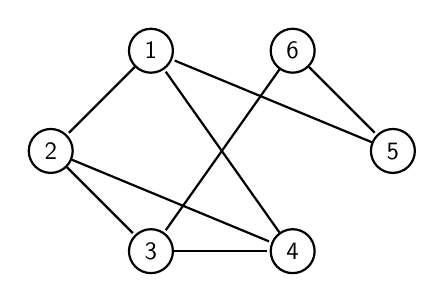
\begin{tikzpicture}[-,>=stealth,shorten >=1pt,auto,node distance=2cm,thick,main node/.style={scale=0.9,circle,draw,font=\sffamily\normalsize}]
            \node[main node] (1) {1};
            \node[main node] (2) [below left of=1] {2};
            \node[main node] (3) [below right of=2] {3};
            \node[main node] (6) [right of=1] {6};
            \node[main node] (5) [below right of=6] {5};
            \node[main node] (4) [below left of=5] {4};

            \path[every node/.style={font=\sffamily\small}]
                (1) edge (2)
                (2) edge (3)
                (2) edge (4)
                (3) edge (4)
                (4) edge (1)
                (5) edge (1)
                (6) edge (3)
                (6) edge (5)
                ;
        \end{tikzpicture}
    \end{figure}
    
    Suppose that we want to describe the property \curlyquotes{every vertex of the graph $G$ has at most 3 neighbors}. Predicate logic allows us to express such property through the use of \textbf{quantifiers} in the following way:
    \[\forall x_t, x_i, x_j, x_k (\lnot E(x_t, x_i) \lor \lnot E(x_t, x_j) \lor \lnot E(x_t, x_k))\]
    
    When the domain is finite, such as this case, the quantifier $\forall$ can be \curlyquotes{simulated} through a conjunction:
    \[\bigwedge_{1 \leq t \leq 6} \bigwedge_{1 \leq i,j,k \leq 6} (\lnot p_{t,i} \lor \lnot p_{t,j} \lor p_{t,k})\]

    obtaining a proposition where we intuitively have that $p_{a,b} = 1$ if and only if $(a,b) \in E$. When the domain is infinite, instead, such simulation cannot be achieved since, by definition, a proposition cannot be infinite. Nonetheless, the above formula can indeed be simulated in propositional logic, but it would require the construction of an infinite theory, which we amply discussed to be not so easy to work with.

    In \textit{predicate logic}, concepts described in terms of relational structures.

    \begin{frameddefn}{Relational structure}
        A \textbf{relational structure} (or \textit{predicate structure}) is a tuple $\mathcal{A} = (A, R_1, \ldots, R_n, c_1, \ldots, c_k)$ where:
        \begin{itemize}
            \item $A$ is a non-empty set called \textit{domain}
            \item $R = \{R_1, \ldots, R_n\}$ are \textit{relations} on $A$ of any arity, even different ones.
            \item $c_1, \ldots, c_k$ are \textit{constants}, i.e. special elements of $A$ that have been \curlyquotes{explicitely named}
        \end{itemize}
    \end{frameddefn}

    For instance, the previous graph can be described as $\mathcal{G} = (V,E)$, where $V = \{1,2,3,4,5,6\}$ is the domain and $E$ is the edge relation.
    \[ E = \{(1,2), (1,4), (1,5), (2,3), (3,4), (3,6), (5,6)\}\]

    We observe that even concepts such as mathematical operations can be described as a relational structure. For instance $\mathcal{N} = (\N, \leq, +, \times, 0,1)$ is a relational structure on the natural numbers where 0 and 1 have been explicitly stated. In other words, we have that $\N = \{n_0, n_1, n_2, \ldots\}$ and we have denoted $n_0$ as 0 and $n_1$ as 1. The operation $+ : \N \times \N \to \N$ can be described through its \textit{operation graph}, i.e. the ternary relation defined as:
    \[+ = \{(n_0, n_1, n_1), (n_0, n_2, n_2), \ldots, (n_1, n_2, n_3), (n_1, n_3, n_4), \ldots\}\]

    where $+(a, b, c)$ if and only if $a + b = c$. Generally, we want to use predicate logic express natural global properties of structures and local properties of elements of structures. For example, for a graph $\mathcal{G} = (V, E)$ we might want to express global properties such as: $\mathcal{G}$ is undirected, $\mathcal{G}$ is complete, \dots. The concept of predicate logic is designed in order to reflect the complexity of what we
    called \textit{structures}. Basically we have one linguistic (syntactical) component corresponding to each (semantic) component of a structure. Besides, we have properly logical syntactical elements such as variables $x_1, \ldots, x_n$, logical connectives $\lnot, \land, \lor, \ldots$, quantifiers $\forall, \exists$ and the identity symbol $=$.

    However, in predicate logic we can quantify \underline{only on elements} of the structure and not on \underline{structures themselves}. This is the reason predicate logic is also called \textbf{First-order logic}. Quantification over structures, instead, is allowed in \textbf{Second-order logic}, while no quantification is allowed in \textbf{Zeroth-order logic}, i.e. propositional logic.

    \begin{frameddefn}{Relational language}
        A \textbf{relational language} (or \textit{predicate language}, \textit{first-order language}) is a tuple $\mathcal{L}$ of symbols of the following types:
        \begin{enumerate}
            \item A countably infinite set of \textit{variables}
            \item A finite or countably infinite set of \textit{relation symbols}, each with its arity
            \item A finite or countably infinite set of \textit{constant symbols}
        \end{enumerate}
    \end{frameddefn}
    
    To properly distinguish between structures and language, we observe that structures are \textbf{instances of a language} -- in programming terms, this can be viewed as the difference between an object and a class. For instance, a possible language for Graph Theory is $\mathcal{L}_{G} = (E)$, where the binary relation symbol $E$ denotes that any structure $\mathcal{G}$ defined on $\mathcal{L}_\mathcal{G}$ has to have a binary relation $E^\mathcal{G}$. This relation varies from instance to instance. 

    From now on, we'll \underline{always assume} that any relational language has the equality symbol $=$. This symbol can be described in two ways:
    \begin{enumerate}
        \item $=$ is a binary relation symbol and any structure over the language instances it as $\{(a_1, a_1), (a_2, a_2), \ldots,\}$
        \item $=$ is a special symbol and any formula over the language always implicitly contains clauses that describe equality
    \end{enumerate}

    The two definitions are equivalently solid, so we'll use both of them -- mostly the first one. In any language, objects of the domain are referred to as \textbf{terms}. By definition, such objects can be variables or constants. 

    Terms with no variables, i.e. constants, are sometimes referred to as \textit{closed terms}. Similarly to predicate logic, formulas are also inductively defined in terms of connectives (and quantifiers in this case).

    \begin{frameddefn}{Formula}
        Given a relational language $\mathcal{L}$, a \textbf{formula} is a finite string $F$ such that one of the following holds: 
        \begin{itemize}
            \item $F$ is the string $R(t_1, \ldots, t_n)$ where $t_1, \ldots, t_n$ are terms of $\mathcal{L}$
            \item $F$ is the string $t_i = t_j$ where $t_i, t_j$ are terms of $\mathcal{L}$
            \item $F$ is the string $\lnot H$, where $H$ is a formula
            \item $F$ is the string $G * H$, where $G,H$ are formulas and $*$ is a boolean connective
            \item $F$ is the string $Q x \; H$ where $H$ is a formula, $x$ is a variable of $\mathcal{L}$ and $Q$ is a quantifier ($\forall, \exists$).
        \end{itemize}
    \end{frameddefn}

    The first two types of formulas are called \textbf{atomic formulas}, while the others are called \textit{non-atomic}. In the last type of formula, $x$ is a \curlyquotes{variable on the variables of $\mathcal{L}$}, referred to as \textbf{metavariable}, while $H$ is referred to as the \textbf{scope} of the quantifier. In other words, if $v_1, v_2, \ldots$ are the variables of $\mathcal{L}$, the formula $\forall x \; H$ expresses that what $H$ says about $x$ has to hold for any variable among $v_1, \ldots, v_2$, while $\exists x \; H$ expresses that it has to hold for at least one variable.
    
    When the scope $H$ contains a variable $v$ that hasn't been quantified, the variable is said to be \textbf{free}, otherwise we say that it is \textbf{bound}. We observe that he same variable can have in the same formula free and bound occurrences. For instance, in the formula $(\forall x \; R(x,x)) \to R(x,x)$ the variable $x$ is bound in the first subformula and free in the second one. A formula without free variables is referred to as \textbf{sentence}.
    
    If $F$ is a formula and $x_1, \ldots , x_n$ are distinct variables, we write $F(x_1, \ldots , x_n)$ to indicate that the free variables of $F$ are contained in the set ${x_1, \ldots , x_n}$. This notation is also useful to deal with \textbf{substitution} of terms for variables: f $F(x_1, \ldots, x_n)$ is a formula and $t_1, \ldots , t_n$ are terms, we denote with $F(t_1, \ldots , t_n)$ (or $F(x_1/t_1, \ldots , x_n/t_n))$ the formula obtained by simultaneously substituting each free occurrence of variable $x_i$ in $F$ with the term $t_i$. For instance, if $F(x_1, x_2, x_3) = R(x_1, x_2) \land R(x_3, x_1)$ and $a,b,c$ are terms of the language then $F(a, b, c) = R(a, b) \land R(a, c)$.

    After defining the syntax of first-order logic, we're ready to define its semantics, i.e. the evaluation of formulas.

    \begin{frameddefn}{$\mathcal{L}$-structure}
        Let $\mathcal{L}$ be a language. An $\mathbf{\mathcal{L}-structure}$ is a structure $\mathcal{A}$ such that:
        \begin{itemize}
            \item $A$ is the domain of $\mathcal{A}$
            \item For each relation symbol $R_i$ in $\mathcal{L}$ there is a relation $R_i^\mathcal{A}$ over $A$ in $\mathcal{A}$
            \item For each constant symbol $c_i$ in $\mathcal{L}$ there is a constant $c_i^\mathcal{A}$ taken from $A$ in $\mathcal{A}$
        \end{itemize}
    \end{frameddefn}

    For the Graph Theory language $\mathcal{L}_{\mathcal{G}} = \{E\}$, any structure $\mathcal{G} = (V, E^\mathcal{G})$ is an $\mathcal{L}_{\mathcal{G}}$-structure. If $E^\mathcal{G}$ is symmetric, the structure $\mathcal{G}$ represents an undirected graph, otherwise it represents a directed graph.

    In this type of logic, the concept of assignment has to be slightly redefined, along with the concept of satisfiability. Let $\model{A}$ be an $\mathcal{L}$-structure. An \textbf{assignment} for $\model{A}$ is a function $\alpha : \mathsf{Vars}_{\mathcal{L}} \to \mathrm{Dom}(\model{A})$.
    
    We say that a formula $F$ is \textbf{satisfied} by $\alpha$ on $\model{A}$, written as $\model{A} \stackrel{\alpha}{\models} F$ or $\model{A} {\models} F[\alpha]$, if one of the following inductive cases holds:
    \begin{itemize}
        \item $F$ is atomic
        \item $F$ is equal to $R(t_1, \ldots, t_n)$ and $(\alpha(t_1), \ldots, \alpha(t_n)) \in R^\model{A}$, where $t_1, \ldots, t_n$ are terms
        \item $F$ is equal to $t_i = t_j$ and $\alpha(t_i) = \alpha(t_j)$ in $\mathcal{L}$, where $t_i, t_j$ are terms
        \item $F$ is equal to $\lnot H$ and $\model{A} \stackrel{\alpha}{\not\models} H$
        \item $F$ is equal to $G * H$ and $(\model{A} \stackrel{\alpha}{\models} G) * (\model{A} \stackrel{\alpha}{\models} H)$, where $*$ is a boolean connective
        \item $F$ is equal to $\forall x \; H$ and for all $s \in \mathrm{Dom}(\model{A})$ it holds that $\model{A} \models G \sbk{\alpha \rmat{x \\ s}}$, where $\alpha \rmat{x \\ s}$ is the assignment obtained by mapping $x \mapsto s$ in $\alpha$
        \item $F$ is equal to $\exists x \; H$ and $\model{A} \stackrel{\alpha}{\not\models} \forall x \; \lnot H$
    \end{itemize}

    We observe that if $F$ is a sentence then $\model{A} \stackrel{\alpha}{\models} F$ doesn't depend on $\alpha$: since there are no free variables, either every assignment satisfies the formula or none does. When a formula is satisfied by every assignment in a structure $\model{A}$, we say that it is \textbf{true} in $\model{A}$, written as $\model{A} \models F$. When a formula is true in every structure, we say that it is a \textbf{tautology} for the language, written as $\models F$. To recap, we have defined four concepts of truthfulness:
    \begin{enumerate}
        \item $\model{A} \stackrel{\alpha}{\models} F$ means that $F$ is true in $\model{A}$ over $\alpha$
        \item $\model{A} \models F$ means that $F$ is true in $\model{A}$ for all $\alpha$, i.e. $\forall \alpha$ it holds that $\model{A} \stackrel{\alpha}{\models} F$
        \item $\models F$ means that $F$ is true in $\mathcal{L}$, i.e. $\forall \model{A}$ it holds that $\model{A}\alpha{\models} F$
    \end{enumerate}

    This definitions of truthfulness easily extend to \textbf{theories}, i.e. set of sentences:
    \begin{itemize}
        \item $\model{A} \models T$ when $\model{A} \models F$ for all $F \in T$
        \item $\models T$ when $\models F$ for all $F \in T$
    \end{itemize}

    We observe that if $F$ is finite then $\model{A} \stackrel{\alpha}{\models} F$ can always be decided through the inductive definition. If $\mathrm{Dom}(\model{A})$ is also finite then $\model{A} \models F$ can also be decided since there are a finite amount of assignments. However, even if $\mathcal{L}$ has a finite number of relation and constant symbols, $\models F$ is only semi-decidable: Even if every structure is finite, there are infinitely possible structures.

    \section{Decision problems for predicate logic}

    After formalizing the three concepts of truthfulness in predicate logic, it's natural to ask if there concepts are treatable under a computational aspect, i.e. if they are decidable.

    We start by considering the \textbf{validity problem}. Given a language $\mathcal{L}$, we say that a sentence $S$ is \textit{valid} (or a \textit{tautology}) in $\mathcal{L}$ if $\models S$. The set of all valid sentences for a language $\mathcal{L}$ is denoted as $\mathsf{Val}_{\mathcal{L}}$. This problem has no algorithmic solutions (not even semi-decidable ones) for almost all non-trivial first-order languages, while it has algorithmic solutions for some restricted languages. We will be also interested in the version of the validity problem restricted to finite models, that is deciding the set of sentences that are true in all finite relational structures. We denote this set by $\mathsf{FinVal}_{\mathcal{L}}$.

    An easier version of this problem is the \textbf{satisfiability problem}. Here, we're interested in deciding if there is an $\mathcal{L}$-structure $\model{A}$ that satisfies a fixed sentence $S$, i.e. $\model{A} \models S$. The set of satisfiable sentences in a language $\mathcal{L}$ is denoted with $\mathsf{Sat}_{\mathcal{L}}$. Even though it is clearly simpler than $\mathsf{Val}_{\mathcal{L}}$, this set is also not semi-decidable.

    What about the easiest type of truth evaluation? The \textbf{model-checking} problem asks to decide if for a structure $\model{A}$, a formula $F$ and an assignment $\alpha$ it holds that $\model{A} \models F[\alpha]$. For infinite structures, the problem is semi-decidable. For finite structures, instead, the problem is decidable. In fact, we observe that structures \curlyquotes{preserve completeness} in predicate logic. In particular, given any assignment $\alpha$, a formula $F$ and a structure $\model{A}$ over $\mathcal{L}$ it holds that:
    \[\model{A} \not\models F[\alpha] \iff \model{A} \models \lnot F[\alpha] \]

    Hence, we can build a recursive algorithm over the inductive definition of $\model{A} \models F[\alpha]$ to decide it. The time complexity of such algorithm is polynomial in the size of the structure and exponential in the size of the formula. The space complexity, instead, is logarithmic in the size of the structure and polynomial in the size of the formula. In fact, the model-checking for first-order can be proven to be $\mathsf{PSPACE}$-complete by reduction from $\mathsf{TQBF}$, i.e. the Totally Quantified Boolean Formulas problem.

    It is natural to consider formulas with free variables as defining subsets of a structure, by looking at the set of assignments that satisfy the formula. From the perspective of Database Theory, this means reading a formula as a query; from a more mathematical perspective this means investigating which subsets of a structure can be defined by formulas in the language. The \textbf{query evaluation} problem formalizes this question: given a structure $\model{A}$ and a formula $F(x_1, \ldots, x_n)$ in $\mathcal{L}$, the problem asks to decide the set $F^{\model{A}}$, defined as:
    \[F^{\model{A}} = \{(a_1, \ldots, a_n) \in A^n \mid \model{A} \models F(a_1, \ldots, a_n)\}\]

    Some structures/databases are more interesting than others. It is therefore natural to fix one such structure and investigate the set of sentences that are true in it. This set of sentences is called \textbf{theory of the structure}.

    \begin{frameddefn}{Theory of a structure}
        Given an $\mathcal{L}$-structure $\model{A}$, the \textbf{theory of $\model{A}$} is the set $\mathrm{Th}(\model{A})$, defined as:
        \[\mathrm{Th}(\model{A}) = \{S \text{ sentence} \mid \model{A} \models S\}\]
    \end{frameddefn}

    The decision problem for theories of particular structures is of fundamental interest in logic, database theory and from a more general mathematical perspective. Depending on the structure $\model{A}$ and the language considered, the problem can have one between the following answers:
    \begin{itemize}
        \item The problem is undecidable
        \item The problem is decidable but unfeasible
        \item The problem is decidable and feasible
    \end{itemize}

    For the particular case of finite structures, the problem is always decidable. The level of computational complexity for this problem is referred to as \textbf{expression complexity} (or \textit{query complexity}). For first-order logic, this complexity is $\mathsf{PSPACE}$.
    
    In some cases, it's interesting to ask the inverse question, i.e. asking which structures are models for a given sentence, equivalent to deciding the set of \textbf{models of a sentence}.

    \begin{frameddefn}{Models of a sentence}
        Given a sentence $S$ and a language $\mathcal{L}$, the \textbf{models of $\mathbf{S}$} is the set $\mathrm{Mod}(S)$, defined as:
        \[\mathrm{Mod}(S) = \{\model{A} \text{ $\mathcal{L}$-structure} \mid \model{A} \models S\}\]
    \end{frameddefn}

    For possibly infinite structures, it might not even make sense to ask for an algorithm to decide membership in $\mathrm{Mod}(S)$, since there are infinitely many of them. For finite structures, instead, such an algorithm always exists and. The level of computational complexity for this problem is referred to as \textbf{structure complexity} (or \textit{data complexity}). For first-order logic, this complexity is $\mathsf{LOGSPACE}$.


    \section{Expressibility and structural isomorphisms}

    Consider a class $\mathcal{C}$ of structures adequate for some language $\mathcal{L}$ (e.g. the class of all graphs, the class of all finite graphs, \dots). Consider now any property $P$ of structures in the class $\mathcal{C}$. This property induces a bipartition on $\mathcal{C}$ through the set of all structures with property $P$ and all those for which $P$ doesn't hold (e.g. $P$ can be the property of being a connected and $\mathcal{C}$ is the class of all simple undirected graphs). We can then ask whether there is a theory $T$ in the language $\mathcal{L}$ which precisely defines the property $P$ over the class $\mathcal{C}$ in the sense described above, i.e. such that for all $\model{A}$ in $\mathcal{C}$ it holds that $\model{A} \models T$ if and only if $P(\model{A})$ holds. If such sentence exists, we say that the property $P$ is \textbf{expressible} in the language $\mathcal{L}$ over the class $\mathcal{C}$.
    
    \begin{frameddefn}{Expressibility}
        Let $\mathcal{L}$ be a language and let $\mathcal{C}$ be a class of $\mathcal{L}$-structures. Given a property $P$, we say that $P$ is \textbf{expressible} (or \textit{definable}, \textit{axiomatizable}) in $\mathcal{L}$ over $\mathcal{C}$ if there is a theory $T$ (a set of sentences) in $\mathcal{L}$ such that:
        \[\forall \model{A} \in \mathcal{C} \;\; \model{A} \models T \iff P(\model{A}) \text{ holds} \]

        If the theory $T$ is finite, we say that $P$ is \textbf{finitely expressible}.
    \end{frameddefn}
    
    The concept of expressibility plays a main role in first-order logic: it corresponds to the fundamental question \curlyquotes{what \underline{can} be said in first order logic?}.

    For instance, consider the property $P$ = \curlyquotes{$\model{A}$ has exactly $p$ elements}. This property can be expressed through the following sentence $S^P$:
    \[S^P \equiv \; \exists x_1 \exists x_2 \ldots \exists x_p \;\; \rbk{\bigwedge_{1 \leq i,j \leq p} \lnot (x_i = x_j)} \land \rbk{\forall y \; \rbk{\bigvee_{1 \leq j \leq p} y = x_j}}\]

    The first series of ANDs expresses that the domain contain at least $p$ distinct elements, while the second series expresses that every additional element must be equal to one of the first $p$ distinct elements.
    
    The use of infinite theories allows us to express concepts that would otherwise be impossible to finitely express in first-order logic. For instance, consider the property $I$ = \curlyquotes{$\model{A}$ has an infinite number of elements}. For any $n \in \N$, let $A_n$ be the property \curlyquotes{$\model{A}$ has at least $n$ elements}. This last property can be expressed with a generalization of the first part of the previous sentence:
    \[S^{A_n} \equiv \; \exists x_1 \exists x_2 \ldots \exists x_n \;\; \bigwedge_{1 \leq i,j \leq n} \lnot (x_i = x_j)\]

    Consider now the following theory $T^I$:
    \[T^I = \{S^{A_n} \mid n \in \N\}\]

    where $S^{A_n}$ is the sentence expressing $A_n$. It's easy to see that:
    \[\model{A} \models T^I \iff I(\model{A}) \text{ holds}\]

    What about the property $\lnot I$ = \curlyquotes{$\model{A}$ has a finite number of elements}? Surprisingly, this simple property is \textbf{inexpressible} in first-order logic! To prove this, we can use the first-order logic version of the \textbf{compactness theorem}, in particular it's second formulation.

    \begin{framedthm}{Compactness theorem in FOL}
        Let $T$ be a FOL theory of finite or countably infinite cardinality. Then, $T$ is satisfiable if and only if it is finitely satisfiable
    \end{framedthm}

    \begin{proof}
        Omitted.
    \end{proof}
    
    We recall that satisfiability in FOL is defined through the existence of a \underline{satisfying structure} for the theory. By way of contradiction, suppose that there is a theory $T^{\lnot I}$ that expresses $\lnot I$. Consider a new theory $T = T^I \cup T^{\lnot I}$. For each finite subset of $T$ we can build an ad-hoc structure that satisfies it, meaning that $T$ is finitely satisfiable. Formally, given a finite subset $S \underset{fin}{\subseteq} T$, consider $S-T^{\lnot I} = \{S^{A_{i_1}}, \ldots, S^{A_{i_k}}\}$. Let $M = \max(i_1, \ldots, i_k)$. Then, the structure $\model{A}$ with exactly $M$ elements satisfies all the sentences in $S-T^{\lnot I}$ and $T^{\lnot I}$, concluding that $S$ is satisfiable. By Compactness, $T$ is finitely satisfiable if and only if it is satisfiable. However, we know that this is absurd since $T$ is clearly unsatisfiable since no structure can be finite and infinite at the same time. Hence, the only possibility is that $T^{\lnot I}$ cannot exist, concluding that $\lnot I$ is inexpressible in first-order logic.

    \newpage

    Consider now the following directed graph:

    \begin{figure}[H]
        \centering

        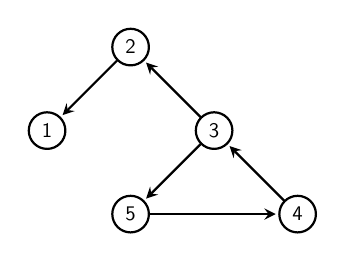
\begin{tikzpicture}[->,>=stealth,shorten >=1pt,auto,node distance=2cm,thick,main node/.style={scale=0.75,circle,draw,font=\sffamily\normalsize}]
            \node[main node] (1) []{1};
            \node[main node] (2) [above right of = 1]{2};
            \node[main node] (3) [below right of = 2]{3};
            \node[main node] (4) [below right of = 3]{4};
            \node[main node] (5) [below left of = 3]{5};

            \path[every node/.style={font=\sffamily\small}]
                (2) edge (1)
                (3) edge (2)
                (3) edge (5)
                (4) edge (3)
                (5) edge (4)
                ;
        \end{tikzpicture}
    \end{figure}

    Let $\mathcal{G} = (V,E)$ be the structure corresponding to the above graph. Given the following sentence $S$ :
    \[\begin{split}
        S \equiv \; & \exists x_1 \exists x_2 \exists x_3 \exists x_4 \exists x_5 \; (E(x_2, x_1) \land E(x_3,x_2) \land E(x_3, x_5) \\
        &\land E(x_4, x_3) \land E(x_5, x_4)) \land \bigwedge_{1 \leq i,j \leq 5} \lnot (v_i = v_j)
    \end{split}\]

    it's easy to see that $\mathcal{G}$ satisfies it. However, the sentence doesn't \textit{exactly describe} $\mathcal{G}$. For instance, this sentence can be also satisfied by any graph extension of $\mathcal{G}$, that being graphs obtained by adding other nodes or edges to $\mathcal{G}$. In expressibility terms, the sentence $S$ defines the property \curlyquotes{$\model{A}$ is a graph with the edges $(v_2,v_1), \ldots, (x_5,x_4)$ for some $v_1, \ldots, v_5$}. 

    To perfectly express $\mathcal{G}$, i.e. build a sentence that defined the property \curlyquotes{$\model{A}$ is the graph $\mathcal{G}$} we have to specify that there are exactly six vertices and which edges do or do not exist between them:
    \[\begin{split}
        S^{\mathcal{G}} \equiv \; & \rbk{\bigwedge_{1 \leq i,j \leq 5} \lnot (x_i = x_j)} \land \rbk{\forall y \; \rbk{\bigvee_{1 \leq j \leq 5} y = x_j}} \\
        &\land  (\lnot E(x_1, x_2) \land \lnot E(x_1, x_3) \land \lnot E(x_1, x_4)  \land \lnot E(x_1, x_5)) \\
        &\land  (E(x_2, x_1) \land \lnot E(x_2, x_3) \land \lnot E(x_2, x_4)  \land \lnot E(x_2, x_5))  \\
        &\land  (\lnot E(x_3, x_1) \land E(x_3, x_2) \land \lnot E(x_3, x_4)  \land E(x_3, x_5)) \\
        &\land  (\lnot E(x_4, x_1) \land \lnot E(x_4, x_2) \land E(x_4, x_3)  \land \lnot E(x_4, x_5)) \\
        &\land  (\lnot E(x_5, x_1) \land \lnot E(x_5, x_2) \land \lnot E(x_5, x_3)  \land E(x_5, x_4))
    \end{split}\]

    However, we observe that $\mathcal{G}$ actually isn't the unique graph satisfying $S^\mathcal{G}$. In fact, any graph $\mathcal{G'}$ obtained by permuting the labels of the vertices of $\mathcal{G}$ also satisfies such sentence. From a mathematical prospective, the two graphs aren't equivalent but they are indistinguishable from each other under a logical level. When this happens, we say that the two structures are \textbf{isomorphic}.

    \begin{frameddefn}{Structural isomorphism}
        Let $\model{A}, \model{B}$ be two $\mathcal{L}$-structures. We say that $\model{A}$ and $\model{B}$ are \textbf{stucturally isomorphic}, written as $\model{A} \cong \model{B}$, when there is a bijective function $h : \mathrm{Dom}(\model{A}) \to \mathrm{Dom}(\model{B})$, called \textbf{isomorphism}, that \textit{preserves truthfulness}, meaning that:
        \begin{itemize}
            \item For each relation symbol $R$ of arity $k$ in $\mathcal{L}$ and for all $(a_1, \ldots, a_n) \in A^n$ it holds that:
            \[(a_1, \ldots, a_n) \in R^{\model{A}} \iff (h(a_1), \ldots, h(a_n)) \in R^{\model{B}}\]
            \item For each constant symbol $c$ in $\mathcal{L}$ it holds that:
            \[c^{\model{A}} = h(c^{\model{B}})\]
        \end{itemize}
    \end{frameddefn}

    Since by definition structural isomorphism preserve truthfulness, it's easy to see that two isomorphic structures always satisfy the same sentences -- it can be formally proven using the inductive definition of satisfiability. This concept is known as \textbf{elementary equivalence} between structures.

    \begin{frameddefn}{Elementary equivalence}
        Let $\model{A}, \model{B}$ be two $\mathcal{L}$-structures. We say that $\model{A}$ and $\model{B}$ are \textbf{elementarily equivalent} in $\mathcal{L}$, written as $\model{A} \equiv_{\mathcal{L}} \model{B}$, when $\mathrm{Th}(\model{A}) = \mathrm{Th}(\model{B})$.
    \end{frameddefn}

    \begin{framedprop}{}
        Let $\model{A}, \model{B}$ be two $\mathcal{L}$-structures. If $\model{A} \cong \model{B}$ then $\model{A} \equiv_{\mathcal{L}} \model{B}$
    \end{framedprop}
    
    The latter proposition implies that any graph that is isomorphic to our example graph $\mathcal{G}$ satisfies $S^{\mathcal{G}}$. However, it's easy to see that this sentence can be satisfied \underline{only} by structures that are isomorphic to $\mathcal{G}$. In other words, the sentence $S^{\mathcal{G}}$ \textbf{characterizes} the graph $\mathcal{G}$ up to isomorphism.

    \begin{framedthm}{Characterizing sentence}
        Let $\model{A}$ be a finite $\mathcal{L}$-structure. Then, there is a sentence $S^{\model{A}} \in \mathrm{Th}(\model{A})$ called \textbf{characterizing sentence} such that for all $\mathcal{L}$-structures $\model{B}$ it holds that:
        \[\model{A} \cong \model{B} \iff \model{B} \models S^{\model{A}}\] 
    \end{framedthm}

    \begin{proof}
        Since $\model{A}$ is finite, we can build a sentence $S^{\model{A}}$ that exactly describes the domain and the relations of $\model{A}$. 
        If $\model{A} \cong \model{B}$, we know that $\model{B} \models S^{\model{A}}$. Vice versa, if $\model{B} \models S^{\model{A}}$ then we know that this can happen only if $\model{A}$ and $\model{B}$ have the same structure. Thus, we can build an isomorphism $h : \mathrm{Dom}(\model{A}) \to \mathrm{Dom}(\model{B})$ by matching the quantifiers of the sentence $S^{\model{A}}$, concluding that $\model{B} \models S^{\model{A}}$.
    \end{proof}

    We observe that the characterizing sentence can be used as a medium to strengthen the previous proposition in the case of finite structures: if the two structures are elementarily equivalent then they will both satisfy the characterizing sentence, which automatically implies that they are isomorphic.

    \begin{framedcor}{}
        Let $\model{A}, \model{B}$ be two finite $\mathcal{L}$-structures. Then, $\model{A} \cong \model{B}$ if and only if $\model{A} \equiv_{\mathcal{L}} \model{B}$
    \end{framedcor}

    For general infinite structures, however, this corollary doesn't always  hold, not even for countably infinite ones. In fact, we'l see that there exist equivalent structures that are not isomorphic. In some cases, however, it is possibile to characterize up to isomorphism a countable structure using sentences.

    \section{The back-and-forth method}

    In the previous section, we discussed how finite structures have a characterizing sentence. For countably infinite theories, we cannot guarantee the existence of such sentence since the trivial sentence describing exactly the structure cannot exist due to the structure being infinite (recall that formulas are finite).
    
    To fix this issue, we can try to extend the concept to theories. The trivial candidate for this task is the set of all the sentences that are satisfiable by a structure, i.e. its theory. In fact, we already stated that if $\model{A} \cong \model{B}$ then $\model{A} \equiv_{\mathcal{L}} \model{B}$, which means that $\mathrm{Th}(\model{A}) = \mathrm{Th}(\model{B})$. Indeed, there are some countably infinite theories for which the contrary implication also holds, even thought not all of them do. We'll see some examples of the latter case in following sections. For now, we'll focus on showing a general approach called the \textbf{back-and-forth method} for proving that elementary equivalence can (sometimes) imply structural isomorphism. 

    Consider the structure $\mathcal{Q} = (\Q, <)$ describing the set of rational numbers $\Q$ and the less than equal relation $<$ over $\Q$. Let $\model{B} = (B, <^{\model{B}})$ be a countably infinite structure such that $\mathrm{Th}(\mathcal{Q}) = \mathrm{Th}(\model{B})$.

    Since both $\mathcal{Q}$ and $\model{B}$ are countably infinite, $\Q$ and $B$ can be enumerated. Let $a_1, a_2, \ldots$ be an enumeration of $\Q$ and let $b_1, b_2, \ldots$ be an enumeration of $B$. The idea is to inductively define two new enumerations $p_1, p_2, \ldots$ and $q_1, q_2, \ldots$ of $\Q$ and $B$ such that the map $h : \Q \to B : p_i \mapsto q_i$ is an isomorphism.

    We start by setting $p_0 = a_0$ and $q_0 = b_0$. For the inductive step, consider a generic $n$ and assume that $p_0, p_1, \ldots, p_n$ and $q_0, q_1, \ldots, q_n$ have been defined. The back-and-forth method splits in two cases: when $n$ is even, we pick a new element from $\Q$ and map it to a new element of $B$, otherwise we pick a new element from $B$ and map it to a new element of $\Q$. The first case is called the \textbf{forth-step}, while the second case is called the \textbf{back-step}.

    First, we observe that since $\mathrm{Th}(\mathcal{Q}) = \mathrm{Th}(\model{B})$, any expressible property that lies in $\mathrm{Th}(\mathcal{Q})$ must be also satisfied by $\model{B}$.
    
    \textit{Forth-step}. Suppose that $n$ is even. Let $p_{n+1}$ be the element in $\Q - \{p_0, p_1, \ldots, p_n\}$ with the smallest possible index in the enumeration $a_0, a_1, \ldots$. By comparing this new element with the previous ones, we have three cases:
    \begin{enumerate}
        \item For all $i \leq n$ we have that $p_{n+1} < p_i$. In this case, we set $q_{n+1}$ as any element in $B$ such that $q_{n+1} <^{\model{B}} q_i$ for all $i \leq n$. The existence of such element $q_{n+1}$ is guaranteed since $\mathrm{Th}(\mathcal{Q})$ contains the sentence expressing \textit{non-minimality}, i.e. $\forall x \exists y \; y < x$
        
        \item For all $i \leq n$ we have that $p_i < p_{n+1}$. In this case, we set $q_{n+1}$ as any element in $B$ such that $q_i <^{\model{B}} q_{n+1}$ for all $i \leq n$. The existence of such element $q_{n+1}$ is guaranteed since $\mathrm{Th}(\mathcal{Q})$ contains the sentence expressing \textit{non-maximality}, i.e. $\forall x \exists y \; x < y$
        
        \item The first two cases do not apply. In this case, there must be two indices $i,j \leq n$ with $i \neq j$ such that $p_i < p_{n+1} < p_j$ and $\nexists k \leq n$ such that $p_i < p_k < p_j$. We set $q_{n+1}$ as any element in $B$ such that $q_i < q_{n+1} < q_j$. The existence of such element $q_{n+1}$ is guaranteed since $\mathrm{Th}(\mathcal{Q})$ contains the sentence expressing \textit{density}, i.e. $\forall x \forall y \; (x < y \to \exists z \; (x < z) \land (z < y))$.
    \end{enumerate}

    In all of the three cases, $q_{n+1}$ is guaranteed to be a new element since $\mathrm{Th}(\mathcal{Q})$ contains the sentence expressing \textit{irreflexivity}, i.e. $\forall x \; \lnot(x < x)$. Moreover, the existence of each relation involving $q_{n+1}$ used in the three cases is guaranteed by the sentences expressing \textit{transitivity} and \textit{totality}, i.e. $\forall x \forall y \forall z ((x < y) \land (y < z) \to x < y)$ and $\forall x \forall y ((x < y) \lor (y < x) \lor (x = y))$.

    \textit{Back-step}. Suppose that $n$ is odd. Let $q_{n+1}$ be the element in $B - \{q_0, q_1, \ldots, q_n\}$ with the smallest possible index in the enumeration $b_0, b_1, \ldots$. The element $p_{n+1}$ is chosen through an argument similar to the three cases of the forth-step.

    Since the back and forth step alternate between each other over each iteration of the inductive process, $\Q$ and $B$ are guaranteed to be fully covered. Moreover, by choice of each next element is easy to see that $h : \Q \to B : p_i \mapsto q_i$ is indeed an isomorphism. This concludes that $\mathcal{Q} \cong \model{B}$. We also notice that the application of the back-and-forth method described above uses only a \textit{restricted theory} of $\mathrm{Th}(\mathcal{Q})$, called \textbf{\textsf{DLO} (Dense Linear Order)}. In fact, the proof shown above works for structure that satisfies this finite theory, concluding that it suffices as a \textbf{characterizing theory} of $\mathcal{Q}$.

    \begin{frameddefn}{Dense Linear Order (\textsf{DLO})}
        We define the \textbf{Dense Linear Order} as the finite theory $\mathsf{DLO}$ containing:
        \begin{enumerate}
            \item \textit{Irreflexivity}: $\forall x \; \lnot(x < x)$
            
            \item \textit{Transitivity}: $\forall x \forall y \forall z ((x < y) \land (y < z) \to x < y)$
            
            \item \textit{Totality}: $\forall x \forall y ((x < y) \lor (y < x) \lor (x = y))$.

            \item \textit{Non-minimality}:
            $\forall x \exists y \; y < x$.

            \item \textit{Non-maximality}:
            $\forall x \exists y \; x < y$.

            \item \textit{Density}: $\forall x \forall y \; (x < y \to \exists z \; (x < z) \land (z < y))$
        \end{enumerate}
    \end{frameddefn}
    
    \begin{framedthm}[label={Q_DLO}]{Characterizing theory of $(\Q, <)$}
        Let $\mathcal{Q} = (\Q, <)$. For any countably infinite structure $\model{B}$ it holds that:
        \[\mathcal{Q} \cong \model{B} \iff \model{B} \models \mathsf{DLO}\]
    \end{framedthm}

    In some cases, the characterizing sentence (or theory) of a class of structures may correspond to a particular property. This is the case of the \textbf{random graph model}, introduced by \textcite{random_graph}. Given a vertex set $V$, a random graph on $V$ is a graph whose edges have a $\frac{1}{2}$ probability of being added to the graph.
    \[\forall \{u,v\} \in \binom{V}{2} \;\; \Pr[\{u,v\} \in E(G)] = \frac{1}{2}\]

    We define the \textit{Random Graph Property} (also known as \textit{Extension Property} or \textit{Alice's Restaurant Property}) as the property stating \curlyquotes{for any pair of disjoint finite subsets $A,B \subseteq V$, there is a vertex outsite of $A$ and $B$ that is connected to all the vertices in $A$ and disconnected from all the vertices in $B$}. This property can be easily expresses in first-order logic through an infinite theory $T = \{S_{n,m} \mid n,m \in \N\}$, where:
    \[\begin{split}
        S_{n,m} \equiv \;& \forall x_1 \ldots \forall x_n \forall y_1 \ldots \forall y_m \; \left ( \bigwedge_{1 \leq i,j \leq n} \lnot(x_i = y_j) \to \right . \\
        &\left . \exists z \; \rbk{\bigwedge_{1 \leq i \leq n} \lnot(z = x_i) \land E(z,x_i)}  \land \rbk{\bigwedge_{1 \leq j \leq n} \lnot(z = y_i) \land \lnot E(z, y_i)} \right )
    \end{split}\]

    Erdős and Rényi were able to prove every sufficiently large random graph satisfies the random graph property $S_{n,m}$ for each $n,m \in \N$ and that every pair of structures satisfying the theory $T$ are isomorphic to each other.

    \begin{framedthm}{Characterizing theory of random graphs}
        Any countable model satisfying the \textit{Random Graph Property} is almost certainly isomorphic to a random graph.
    \end{framedthm}

    \begin{proof}
        First, we prove that any sufficiently large random graph almost certainly satisfies the property. Fix a pair of disjoint finite subsets $A,B \subseteq V$ and fix a vertex $v \in V-(A \cup B)$. Let $\abs{V} = k \abs{A} =n$ and $\abs{B} = m$. Let $Q_v$ be the event \curlyquotes{$N(v) \subseteq A \land N(v) \cap B = \varnothing$}. We observe that:
        \[\Pr[\lnot Q_v] = 1- \Pr[Q_v] = 1 - \rbk{\frac{1}{2}}^n \rbk{\frac{1}{2}}^m = 1-\frac{1}{2^{n+m}}\]
        
        Hence, we have that:
        \[\Pr[\forall v \in V-(A \cup B) \; \lnot Q_v] = \rbk{1- \frac{1}{2^{n+m}}}^{k-n-m}\]

        Since not all finite subsets $A$ of $n$ elements and finite subsets $B$ of $m$ elements are disjoint and there are at most $k^{n+m}$ pairs of subsets, the probability of $S_{n,m}$ not being satisfied is lower bounded by:
        \[\Pr[S_{n,m}] = 1-\Pr[\lnot S_{n,m}] = 1-\Pr[\exists A,B \; \forall v \in V-(A \cup B) \lnot Q_v] \geq 1- k^{n+m} \rbk{1- \frac{1}{2^{n+m}}}^{k-n-m}\] 

        For sufficiently large random graphs, we conclude that:
        \[\lim_{k \to +\infty } \Pr[S_{n,m}] \geq \lim_{k \to +\infty } 1- k^{n+m} \rbk{1- \frac{1}{2^{n+m}}}^{k-n-m} = 1\]

        For the second part, let $\model{A} = (A, E^{\model{A}})$ and $\model{B} = (B, E^{\model{B}})$ be two structures satisfying the random graph property. Let $n = \abs{A} = \abs{B}$. We'll prove that these two structures are isomorphic through a back-and-forth argument. Let $a_1, a_2, \ldots$ be an enumeration of $A$ and let $b_1, b_2, \ldots$ be an enumeration of $B$. We start by setting $p_0 = a_0$ and $q_0 = b_0$. For the inductive step, consider a generic $n$ and assume that $p_0, p_1, \ldots, p_n$ and $q_0, q_1, \ldots, q_n$ have been defined.

        \textit{Forth-step}. Suppose that $n$ is even. Let $p_{n+1}$ be the element in $A - \{p_0, p_1, \ldots, p_n\}$ with the smallest possible index in the enumeration $a_0, a_1, \ldots$. We split $\{p_0, p_1, \ldots, p_n\}$ into two two disjoint subsets according to the connectedness on $p_{n+1}$:
        \[X = \{i \mid i \leq n, (p_i, p_{n+1} \in E^{\model{A}})\}\]
        \[Y = \{j \mid j \leq n, (p_j, p_{n+1} \notin E^{\model{A}})\}\]

        Consider now the subsets $X',Y'$ of $H$ induced by $X,Y$:
        \[X' = \{q_i \mid p_i \in X\}\]
        \[Y' = \{q_j \mid p_j \in Y\}\]

        By construction of the inductive process, since $X,Y$ are disjoint $X',Y'$ must also be disjoint. Hence, since $\model{B}$ satisfies the random graph property and the premise of the axiom $S_{\abs{X'}, \abs{Y'}}$, its consequence must also be satisfied, meaning that there is a vertex $v \in B-(X' \cup Y')$ that is adjacent to every vertex in $X'$ and disconnected from each vertex in $Y'$. We fix $q_{n+1} = v$.

        \textit{Back-step}. Suppose that $n$ is odd. Let $q_{n+1}$ be the element in $B - \{q_0, q_1, \ldots, q_n\}$ with the smallest possible index in the enumeration $b_0, b_1, \ldots$. The element $p_{n+1}$ is chosen through an argument similar to the  forth-step.

        Since the back and forth step alternate between each other over each iteration of the inductive process, $\Q$ and $A$ are guaranteed to be fully covered. Moreover, by choice of each next element is easy to see that $h : A \to B : p_i \mapsto q_i$ is indeed an isomorphism. This concludes that $\model{A} \cong \model{B}$.
    \end{proof}

    \section{Bounded equivalence}

    Elementary equivalence can be used to prove non-expressibility results: if two structures $\model{A}$ and $\model{B}$ are elementarily equivalent but only one of them has the property $P$ then the only possibility is that the property $P$ cannot be expressed in first-order logic, since otherwise it would lie inside both $\mathrm{Th}(\model{A})$ and $\mathrm{Th}(\model{B})$.

    \begin{framedprop}{First method for non-expressibility in FOL}
        Let $P$ be a property for a class of structures $\mathcal{C}$. Then, $P$ is not expressible in FOL if there are two structures $\model{A}, \model{B}$ such that $\model{A} \equiv \model{B}$ but they don't share the property $P$.
    \end{framedprop}

    However, we observe that this method for proving non-expressibility fails for finite models: we proved that in this case elementary equivalence implies that the two structures are isomorphic, meaning that the two models cannot differ by any sensible property $P$ (as long as $P$ is preserved under isomorphisms, a standard assumption in both \textit{Mathematics} and \textit{Computer Science}). To overcome this problem, we will consider a \textit{graded} version of elementary equivalence, i.e. \textbf{bounded elementary equivalence}, which expresses the idea that two structures cannot be distinguished by sentences of a specific syntactic complexity. For instance, consider the following two graphs:
    \begin{figure}[H]
        \centering

        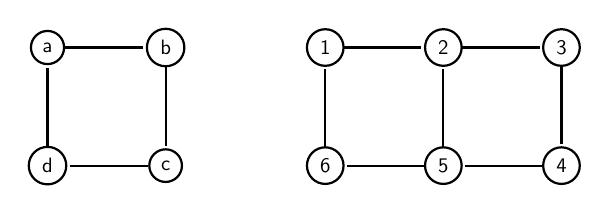
\begin{tikzpicture}[-,>=stealth,shorten >=1pt,auto,node distance=2cm,thick,main node/.style={scale=0.75,circle,draw,font=\sffamily\normalsize}]
            \node[main node] (1) []{a};
            \node[main node] (2) [right of = 1]{b};
            \node[main node] (3) [below of = 2]{c};
            \node[main node] (4) [left of = 3]{d};

            \node[main node] (5) [right of = 2, xshift = 20]{1};
            \node[main node] (6) [right of = 5]{2};
            \node[main node] (7) [right of = 6]{3};
            \node[main node] (8) [below of = 7]{4};
            \node[main node] (9) [left of = 8]{5};
            \node[main node] (10) [left of = 9]{6};


            \path[every node/.style={font=\sffamily\small}]
                (1) edge (2)
                (2) edge (3)
                (3) edge (4)
                (4) edge (1)

                (5) edge (6)
                (6) edge (7)
                (7) edge (8)
                (8) edge (9)
                (9) edge (6)
                (9) edge (10)
                (10) edge (5)
                ;
        \end{tikzpicture}
    \end{figure}

    Many sentences are able to distinguish the two graphs, such as:
    \begin{enumerate}
        \item The sentence expressing \curlyquotes{there is a node with at least three neighbors}
        \[\exists x_1 \exists x_2 \exists x_3 \exists x_4 \bigwedge_{i,j} \lnot (x_i = x_j) \land E(x_1, x_2) \land E(x_1, x_3) \land E(x_1, x_4)\]

        is satisfied only by the second graph.

        \item The sentence expressing \curlyquotes{there are three nodes that are independent}
        \[\exists x_1 \exists x_2 \exists x_3 \bigwedge_{i,j} \lnot (x_i = x_j) \land \lnot E(x_i, x_j)\]
        is satisfied only by the second graph.
    \end{enumerate}

    After some trial and error, we can convince ourselves that there seem to be no sentence with less than three quantifiers that is able to distinguish the two graphs: after fixing two nodes through two quantifiers, we require at least another quantifier to express any property. This fact can be formally proven, meaning that we strictly require at least three quantifiers to distinguish the two graphs. This gives us some notion of \textit{syntactic complexity} for predicate formulas: the \textbf{quantifier rank} of a formula. 

    \begin{frameddefn}{Quantifier rank}
        Let $F$ be a formula. The \textbf{quantifier rank} (or \textit{degree}) of $F$, written as $\rk(F)$, is inductively defined as:
        \begin{itemize}
            \item If $F$ is an atomic formula then $\rk(F) = 0$
            \item If $F = G * H$ for some boolean connective $*$ then $\rk(F) = \max(\rk(G), \rk(H))$
            \item If $F = \lnot H$ then $\rk(F) = \rk(H)$
            \item If $F = Q x_1 \lnot H$ for some quantifier $Q$ then $\rk(F) = \rk(H) + 1$
        \end{itemize}
    \end{frameddefn}

    We denote with $\mathrm{Th}_k(\model{A})$ the set of all sentences of rank at most $k$ that are satisfied by $\model{A}$. As we discussed, the two previous example graphs satisfy the same sentences up to two quantifiers. This is known as $2$-elementary equivalence. 

    \begin{frameddefn}{$k$-elementary equivalence}
        Let $\model{A}, \model{B}$ be two $\mathcal{L}$-structures. We say that $\model{A}$ and $\model{B}$ are \textbf{$k$-elementarily equivalent} in $\mathcal{L}$, written as $\model{A} \equiv_{k} \model{B}$, when $\mathrm{Th}_k(\model{A}) = \mathrm{Th}_k (\model{B})$.
    \end{frameddefn}

    By definition, it holds that every structure for the same language is $0$-equivalent and that $\model{A} \equiv_{k} \model{B}$ for all $k \in \N$ if and only if $\model{A} \equiv \model{B}$. The notion of $k$-elementary equivalence gives rise to a method for proving non-expressibility of queries over finite models. Suppose that a property $P$ is \textit{finitely axiomatizable}, meaning that there is a sentence expressing it. Then, the axioms have some maximal quantifier rank $k$. If we show that for any $k$ there are two structures that don't share $P$ but satisfy the same sentences up to that complexity then $P$ is not finitely axiomatizable.

    \begin{framedprop}[label={non_exp_2}]{Second method for non-expressibility in FOL}
        Let $P$ be a property for a class of structures $\mathcal{C}$. Then, $P$ is not finitely expressible in FOL if for all $k \in \N$ there are two structures $\model{A}, \model{B}$ such that $\model{A} \equiv_k \model{B}$ but they don't share the property $P$.
    \end{framedprop}

    This method clearly works for both finite and non-finite structures, making it of interest to isolate methods for proving that $\model{A} \equiv_k \model{B}$. One such method was given by \textcite{fraisse}, who used the back-and-forth method on \textbf{structure expansions}.
    
    \begin{frameddefn}{Structure expansion}
        Let $\model{A}$ be an $\mathcal{L}$-structure and let $c_1, \ldots, c_n$ be new constant symbols. Let $\mathcal{L}^c = \mathcal{L} \cup \{c_1, \ldots, c_n\}$. Given $a_1, \ldots, a_n \in A$, the \textbf{expansion} of $\model{A}$ over $a_1, \ldots, a_n$, written as $(\model{A}, a_1, \ldots, a_n)$, is the $\mathcal{L}^c$-structure that coincides with $\model{A}$ and interprets $c_i$ as $a_i$. 
    \end{frameddefn}

    We observe that the language $\mathcal{L}^c$ for structure $(\model{A}, a_1, \ldots , a_n)$ contains more sentences (in particular more atomic ones) than language $\mathcal{L}$. In general, if $F(x_1, \ldots, x_n)$ is a formula of $\mathcal{L}$, we denote with $F^c$ the $\mathcal{L}^c$ formula obtained by substituting each $x_i$ with $c_i$. By definition, we have that:
    \[(\model{A}, a_1, \ldots, a_n) \models F^c \iff \model{A} \models F(x_1, \ldots, x_n)[a_1, \ldots, a_n]\]

    To make things clearer, we illustrate an example. Consider the language $\mathcal{L} = \{U(x),$ $M(x, y), P(x, y)\}$. Let $\model{A} = (A, U^{\model{A}}, M^{\model{A}}, P^{\model{A}})$ be a structure representing a database with a finite domain of individuals, i.e. $A = \{\text{George, Mary, \dots, Lisa} \}$, where $U^{\model{A}}$ is the relation of \textit{male individuals}, $M^{\model{A}}$ is the relation of \textit{married individuals} and $P^{\model{A}}$ is the relation of \textit{parent individuals}. We expand the language $\mathcal{L}$ with the new constants $c_1, c_2$. While there are no atomic sentences in the original language, the following are atomic sentences in the
    expanded language $\mathcal{L}^c$: $U(c_1), U(c_2), M(c_1, c_2), M(c_2,c_1), S(c_2, c_1), \ldots$

    Consider now the following formula in $\mathcal{L}$:
    \[F(x_1, x_2) \equiv \exists x_3 \; P(x_1, x_3) \land P(x_2, x_3) \land M(x_1,x_2) \land U(x_3)\]
    
    In the new language, this formula becomes:
    \[F^c \equiv \exists x_3 \; P(c_1, x_3) \land P(c_2, x_3) \land M(c_1,c_2) \land U(x_3)\]

    Fix two individuals in $A$, say George and Lisa ($G, L$ for short). The formula $F^c$ is true in the expansion of $(\model{A}, G,L)$ if and only if $G$ and $L$ are married and they have a common son, which is true if and only if $F(x_1,x_2)[G,L]$ is true in  $\model{A}$.

    \begin{framedthm}[label={fraisse}]{Fraïssé's theorem}
        Let $\model{A}, \model{B}$ be two $\mathcal{L}$-structures. For all $k \geq 0$, it holds that $\model{A} \equiv_{k+1} \model{B}$ if and only if the two following conditions hold:
        \begin{enumerate}
            \item \textit{Forth condition}: for all $a \in A$ there is a $b \in B$ such that $(\model{A}, a) \equiv_k (\model{B}, b)$
            \item \textit{Back condition}: for all $b' \in B$ there is a $a' \in A$ such that $(\model{A}, a') \equiv_k (\model{B}, b')$
        \end{enumerate}
    \end{framedthm}

    \begin{proof}
        First, we observe that any formula of the form $\forall x G(x)$ can be rewritten as $\lnot(\exists x \lnot G(x))$. We also observe that any formula can be written in \textit{prefix form}, meaning that all the quantifiers appear at the start of the formula. Hence, we can restrict our interest of formulas of the form $\exists x F(x)$ of rank at most $k$ and with one free variable $x$.

        Assume that the forth and back conditions hold. Suppose that $\model{A} \models \exists x F(x)$. Then, for some $a \in A$ it must hold that $\model{A} \models F(x)[a]$, which can happen if and only if $(\model{A}, a) \models F^c$. By the forth condition, there must be some $b \in B$ such that $(\model{B}, b) \models F^c$, which can happen if and only if $\model{B} \models F(x)[b]$, concluding that $\model{B} \models \exists x F(x)$. Using the back condition and the same argument, we get that $\model{B} \models \exists x F(x)$ implies $\model{A} \models \exists x F(x)$. Thus, the two structures satisfy the same formulas of rank at most $k+1$, concluding that $\model{A} \equiv_{k+1} \model{B}$.

        Vice versa, assume that $\model{A} \equiv_{k+1} \model{B}$. We prove that the forth condition holds (the back condition follows the same argument). Fix $a \in A$. We notice that the sentences of rank at most $k$ in the language $\mathcal{L}^c$ either contain the new constant $c$ -- meaning that they are of the form $F^c$ for some $F$ in $\mathcal{L}$ with rank at most $k$ -- or they don't contain it -- meaning that they are also in $\mathcal{L}$. In the second case, there is nothing to prove so we assume to be working with the first case.
        
        For a generic structure $\model{D}$ and a value $d \in D$, we define the \textit{$k$-type of $d$ in $\model{D}$}, written as $Q_{\model{D}, d}$, set of formulas with one free variable, rank at most $k$ and that are satisfied by $\model{D}$ with assignment $x \mapsto d$.
        \[Q_{\model{D}, d} = \{F(x) \mid \rk(F(x)) \leq k, \model{D} \models F(x)[d]\}\]
        
        \textbf{Claim 1}: There is a formula $H_{\model{D}, d}(x)$ of rank at most $k$ and with one free variable $x$ that exactly describes $Q_{\model{D}, d}$.

        \begin{proof}[Proof of Claim 1.]
            Let $Q$ be the set of formulas with one free variable and rank at most $k$.
            \[Q = \{F(x) \mid \rk(F(x)) \leq k\}\]

            We observe that $Q$ is finite modulo logical equivalence, meaning that we can consider an unique representative formula for every pair of formulas satisfied by the same assignments. Let $X = \{G_1(x), \ldots, G_m(x)\}$ be the set of such representative formulas. Since $Q_{\model{D}, d} \subseteq Q$, it can be represented by a subset $X_{\model{D}, d} = \{G_{i_1}(x), \ldots, G_{i_t}(x)\}$ of $X$. Let $I = \{i_1, \ldots, i_t\}$. Since $I$ and $\overline{I}$ are finite, we can express through a single formula $H_{\model{D}, d}(x)$ the fact that $x$ satisfies all and only the formulas in $X_{\model{D}, d}$.
            \[H_{\model{D}, d}(x) \equiv \bigwedge_{i \in I} G_i \land \bigwedge_{j \in \overline{I}} \lnot G_j\]
            
            Since each formula of $X$ has rank at most $k$, $H_{\model{D}, d}(x)$ is a formula of degree at most $k$ with one free variable $x$.
        \end{proof}

        Through the first claim, we're able to encode a whole $k$-type into a single formula: proving that another structure satisfies such formula is equivalent to proving that the $k$-type of the initial structure.
        
        \textbf{Claim 2:} There is a $b \in B$ such that $Q_{\model{A},a} = Q_{\model{B},b}$.

        \begin{proof}[Proof of the Claim 2.]
            By construction, we clearly have that $\model{A} \models H_{\model{A},a}(x)[a]$, which can happen if and only if $\model{A} \models \exists x H_{\model{A},a}(x)$. Since $\model{A} \equiv_{k+1} \model{B}$ by hypothesis, we get that $\model{B} \models \exists x H_{\model{A},a}(x)$, which can happen if and only if for some $b \in B$ we have that $\model{B} \models H_{\model{A},a}(x)[b]$, which can happen if and only if $Q_{\model{A},a} = Q_{\model{B},b}$.
        \end{proof}

        Consider now any sentence $F^c$ in $\mathcal{L}^c$ with rank at most $k$ and suppose that $(\model{A},a) \models F^c$. Then, we know that this happens if and only if $\model{A} \models F(x)[a]$, meaning that $F(x) \in Q_{\model{A},a} = Q_{\model{B},b}$, which happens if and only if $(\model{B},b) \models F^c$. 
    \end{proof}

    \section{Ehrenfeucht-Fraïssé games}

    The combinatorial characterization established by Fraïssé's theorem gives us a tool to reason on $k$-elementary equivalence. However, this tool is often impractical and very inconvenient since it basically requires a back-and-forth argument. Building on Fraïssé's result, \textcite{ehrenfeucht} was able to establish a more convient characterization in terms of a two player game, the now called \textbf{Ehrenfeucht-Fraïssé game} (or \textit{Duplicator-Spoiler game}). Given two structures $\model{A}$ and $\model{B}$, on every round the first player -- the \textit{Spoiler} -- picks an element from either $\model{A}$ or $\model{B}$ and the second player -- the \textit{Duplicator} -- has to answer with an element in the other structure so
    that the sequence of choices defines a \textit{partial isomorphism}.

    \begin{frameddefn}{Partial isomorphism}
        Let $\model{A}, \model{B}$ be two structures and let $a_1, \ldots , a_n \in A$ and $b_1, \ldots , b_n \in B$. The partial map $a_1 \mapsto b_1, \ldots, a_n \mapsto b_n$ is said to be a \textbf{partial isomorphism} between $\model{A}$ and $\model{B}$ when:
        \begin{enumerate}
            \item For all $i,j \leq n$ it holds that $a_i = a_j$ if and only if $b_i = b_j$
            \item For all $i \leq n$ it holds that $a_i = c$ if and only if $b_i = c$
            \item For every relation symbol $R$, for all $i_1, \ldots, i_k \in [n]$ it holds that $(a_{i_1}, \ldots, a_{i_k}) \in R^{\model{A}}$ if and only if $(b_{i_1}, \ldots, b_{i_k}) \in R^{\model{B}}$
        \end{enumerate}
    \end{frameddefn}
    
    After $k$ rounds of the game, the two players will have built two sequences $a_1, \ldots , a_k$ of elements of $A$ and $b_1, \ldots , b_k$ of $B$. The Duplicator wins the if the map $a_i \mapsto b_i$ preserves equality and relations, otherwise the Spoiler wins. When the Duplicator has a \textbf{strategy} to win all games of at most $k$ rounds, we say that they win the $k$-round game, otherwise we say that the Spoiler wins the $k$-round game. We denote the $k$-round game on $\model{A}, \model{B}$ with $G_k(\model{A}, \model{B})$.

    We observe that if $\model{A} \cong \model{B}$ are isomorphic then the Duplicator wins the $k$-game for any possible $k \in \N$ since they always have an adequate answer due to the two structures being indistinguishable from each other. Vice versa, if the Duplicator is able to win the $n$-game, with $\abs{A} = \abs{B} = n$, then $\model{A} \cong \model{B}$ since the partial isomorphism defined by the game covers the whole set.

    To give a concrete example, consider again the following two example graphs.
    \begin{figure}[H]
        \centering

        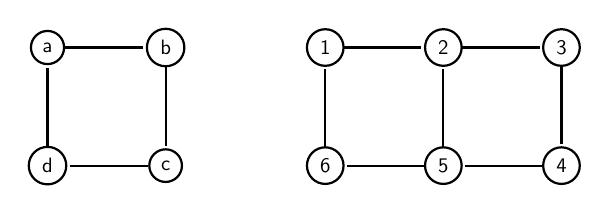
\begin{tikzpicture}[-,>=stealth,shorten >=1pt,auto,node distance=2cm,thick,main node/.style={scale=0.75,circle,draw,font=\sffamily\normalsize}]
            \node[main node] (1) []{a};
            \node[main node] (2) [right of = 1]{b};
            \node[main node] (3) [below of = 2]{c};
            \node[main node] (4) [left of = 3]{d};

            \node[main node] (5) [right of = 2, xshift = 20]{1};
            \node[main node] (6) [right of = 5]{2};
            \node[main node] (7) [right of = 6]{3};
            \node[main node] (8) [below of = 7]{4};
            \node[main node] (9) [left of = 8]{5};
            \node[main node] (10) [left of = 9]{6};


            \path[every node/.style={font=\sffamily\small}]
                (1) edge (2)
                (2) edge (3)
                (3) edge (4)
                (4) edge (1)

                (5) edge (6)
                (6) edge (7)
                (7) edge (8)
                (8) edge (9)
                (9) edge (6)
                (9) edge (10)
                (10) edge (5)
                ;
        \end{tikzpicture}
    \end{figure}

    Suppose that the Spoiler starts the first round by playing the node $2$. To preserve the partial isomorphism, the Duplicator answers with the node $a$, trivially winning the first round since there are no unary relations to be satisfied and no equality constraints to check. For the second round, suppose that the Spoiler plays the node $c$. If the Duplicator answers with the node $6$, they also win the second round since $a \neq c$, $2 \neq 6$ and $(b,d) \notin E^{\mathcal{G}_1}, (2,6) \notin E^{\mathcal{G}_2}$. For the third round, suppose that the Spoiler plays the node $4$. Then, the Duplicator has no way to answer while also preserving the partial isomorphism: if he answers with $b$ then we have $(a,b), (b,c) \in E^{\mathcal{G}_1}$ but $(2,4), (4,6) \notin E^{\mathcal{G}_2}$, while if he answers with $d$ then we have $(a,d), (d,c) \in E^{\mathcal{G}_1}$ but $(2,4), (4,6) \notin E^{\mathcal{G}_2}$.
    
    Thus, there is a strategy for the Spoiler to win the $3$-round game. Moreover, it can be easily proven that the Duplicator always has a strategy to win every single $2$-round game. This has an interesting correspondence with the quantifier complexity of sentences distinguishing $\mathcal{G}_1$ from $\mathcal{G}_2$: we already notices that they can be distinguished by a sentence of rank at least $3$, meaning that $\mathcal{G}_1 \not\equiv_3 \mathcal{G}_2$, but the two structures cannot be distinguished by a sentence of smaller quantifier rank, meaning that $\mathcal{G}_1 \equiv_2 \mathcal{G}_2$.

    \begin{framedlem}{}
        Let $\model{A}, \model{B}$ be two structures and let $a_1, \ldots , a_n \in A$ and $b_1, \ldots , b_n \in B$. Then, for any $k \geq 1$, the Duplicator wins the $k$-game on $(\model{A}, a_1, \ldots, a_n)$ and $(\model{B}, b_1, \ldots, b_n)$ if and only if the following two conditions hold:
        \begin{enumerate}
            \item For all $a \in A$ there is a $b \in B$ such that the Duplicator wins the $(k-1)$-game on $(\model{A}, a_1, \ldots, a_n, a)$ and $(\model{B}, b_1, \ldots, b_n, b)$
            \item For all $b' \in B$ there is a $a' \in B$ such that the Duplicator wins the $(k-1)$-game on $(\model{A}, a_1, \ldots, a_n, a')$ and $(\model{B}, b_1, \ldots, b_n, b')$
        \end{enumerate}
    \end{framedlem}

    \begin{proof}
        Suppose that the Duplicator wins the $k$-game on $(\model{A}, a_1, \ldots, a_n)$ and $(\model{B}, b_1, \ldots, b_n)$. On the first round, the Spoiler can play any $a \in A$ (or any $b \in B$). Since $k \geq 1$, the Duplicator has always an answer $b \in B$ (or $a \in A$) that maintains the partial isomorphism. For any pair $(a, b)$ chosen on the first round, the sequences $a_1, \ldots, a_n, a \mapsto b_1, \ldots, b_n, b$ form a partial isomorphism. Thus, the Duplicator has a strategy to win the $(k-1)$ game on $(\model{A}, a_1, \ldots, a_n, a)$ and $(\model{B}, b_1, \ldots, b_n, b)$, hence the first condition holds. The second condition holds through an analogous argument.

        Vice versa, suppose that the two conditions holds. Then, for any choice $a \in A$ (or $b \in B$) of the Spoiler, the Duplicator can pick an element $b \in B$ (or $a \in A$) that allows him to win the $k-1$ game on $(\model{A}, a_1, \ldots, a_n, a)$ and $(\model{B}, b_1, \ldots, b_n, b)$. The first round is one through the pair $(a,b)$, while the other $k-1$ rounds are won through the same strategy that allows him to win the $k-1$ game.
    \end{proof}

    It's easy to see that the above lemma is very similar to Fraïssé's theorem. In fact, Ehrenfeucht was able to extend the lemma in order to prove that his game characterization is equivalent to the combinatorial charaterization.

    \begin{framedthm}[label={spoil_dup_game}]{Ehrenfeucht's theorem}
        Let $\model{A}, \model{B}$ be two $\mathcal{L}$-structures. For all $k \geq 0$, it holds that $\model{A} \equiv_{k} \model{B}$ if and only if the Duplicator wins $G_k(\model{A}, \model{B})$.
    \end{framedthm}

    \begin{proof}
        We proceed by induction. Suppose that the Duplicator wins the 0-game. Then, this happens if and only if there is a partial isomorphism $h : c^{\model{A}} \mapsto c^{\model{B}}$ on the constant symbols. By definition of partial isomorphism, for each set of constants $c_{i_1}, \ldots, c_{i_k}$ we have that $(c_{i_1}^{\model{A}}, \ldots, c_{i_k}^{\model{A}}) \in R^{\model{A}}$ iff $(c_{i_1}^{\model{B}}, \ldots, c_{i_k}^{\model{B}}) \in R^{\model{B}}$ and $c_i^\model{A} = c_j^{\model{A}}$ iff $c_i^\model{B} = c_j^{\model{B}}$. Hence, $\model{A}$ and $\model{B}$ satisfy the same atomic sentences. Since all rank 0 sentences are atomic, we conclude that $\model{A} \equiv_0 \model{B}$. Vice versa, if $\model{A} \equiv_0 \model{B}$, we can create a partial isomorphism on the constant using the equivalences induced by the atomic sentences, thus the Duplicator always wins the 0-game.

        Assume that the theorem holds for all $m \leq k$ and consider the case $k+1$. By the previous lemma, the Duplicator wins $G_{k+1}(\model{A}, \model{B})$ if and only if the following two conditions hold:
        \begin{itemize}
            \item For all $a \in A$ there is a $b \in B$ such that the Duplicator wins the $k$-game on $(\model{A},a)$ and $(\model{B},b)$
            \item For all $b' \in B$ there is a $a' \in A$ such that the Duplicator wins the $k$-game on $(\model{A},a')$ and $(\model{B},b')$
        \end{itemize}

        By inductive hypothesis, these two conditions are equivalent to:
        \begin{itemize}
            \item For all $a \in A$ there is a $b \in B$ such that the Duplicator wins the $k$-game on $(\model{A}, a) \equiv_k (\model{B},b)$
            \item For all $b' \in B$ there is a $a' \in A$ such that the Duplicator wins the $k$-game on $(\model{A}, a') \equiv_k (\model{B},b')$
        \end{itemize}

        Finally, by \Cref{fraisse}, this can happen if and only if $\model{A} \equiv_{k+1} \model{B}$.
    \end{proof}

    \subsection{Non-expressibility results}

    After proving that the Ehrenfeucht-Fraïssé games can be used to decide the $k$-equivalence between two structures, we'll show some examples on how to apply the game in order to prove that a property is non-expressible in first-order logic.

    \begin{framedprop}{}
        The Even Cardinality query is not first-order definable over the language of Graph Theory.
    \end{framedprop}

    \begin{proof}
        By way of contradiction, suppose that the query is expressible by the sentence $S$. Then, since the expression is finite, it must have a quantifier rank. Let $\rk(S) = k$.  Let $\model{A}$ and $\model{B}$ respectively be the to totally disconnected graphs with $k+1$ and $k+2$ nodes. It's easy to see that the Delayer can win $G_{k}(\model{A}, \model{B})$ since the only relation that has to be preserved is the total disconnection. By \Cref{spoil_dup_game}, this concludes that $\model{A} \equiv_k \model{B}$. However, if $k$ is even then $k+1$ is odd and $k+2$ is even, otherwise $k+1$ is even and $k+2$ is odd. Hence, only one between $\model{A}$ and $\model{B}$ can satisfy $S$, raising a contradiction.
    \end{proof}

    We observe that the fact that the $EC$ query is not expressible over finite graphs does not imply that it cannot be defined over another class of structures. In particular it does not imply that the query is not definable over a smaller class of structures: restricting the class could give more chances of expressing a property. For example, the above proof does not rule out that the query is not definable over the class of graphs that are not totally disconnected, since the structures used in the proof would not belong to that smaller class of structures. We'll now focus on a more complex example, showing that the Even Cardinality query also doesn't hold in the class of finite linear orders.

    \begin{framedprop}{}
        Given $k > 0$, if $\model{A}$ and $\model{B}$ are two linear orders with at least $2^k$ elements then $\model{A} \equiv_k \model{B}$.
    \end{framedprop}

    \begin{proof}
        To prove this, we show that the Duplicator has a winning strategy for the game with $k$ moves on $\model{A}$ and $\model{B}$. To make the proof easier to read, we extend the language with two constant symbols that denote the minimum and the maximum of the linear order, i.e. the first and last element of the order. This extension of the language is equivalent to assuming that the Duplicator plays the minimum in one structure if the Spoiler plays the minimum in the other structure, and similarly for the maximum. It's easy to see that this assumption is solid: in order for the Duplicator to survive, the minimum must always be mapped to the minimum (and similarly for the maximum) since otherwise the Spoiler immediately wins the next round by asking for a predecessor of the minimum (or a successor of the maximum). Hence, we assume that these two moves are played in the first two rounds.

        Let $a_{-1}, a_0$ and $b_{-1}, b_0$ be the interpretations in $\model{A}$ and in $\model[B]$ of min and max. Let $d$ be a distance function on the order, i.e. $d(x, y) = \abs{x - y}$. If $d(x, y) < n$ we say that they are \textit{$n$-close}. Let $B_{n}(x) = \{y \mid d(x, y) < n\}$ be the set of elements that are $n$-close from $y$.

        Fix a round $i \in \N$. Let $a_1, \ldots, a_i$ be the elements played in $\model{A}$ after move $i$ and let $b_1, \ldots, b_i$ be the corresponding elements player in $\model{B}$.
        
        \textbf{Claim}: the Duplicator has a strategy such that, after every $i$-th round of the game, for every $-1 \leq p,q \leq i$ the following three points are satisfied:
        \begin{enumerate}
            \item If $a_q$ is $2^{k-i}$-close $a_p$ then $d(b_p, b_q) = d(a_p, a_q)$
            \item If $a_q$ is not $2^{k-i}$-close $a_p$ then $d(b_p, b_q) \geq 2^{k-1}$
            \item $a_p < a_q$ iff $b_p < b_q$ and $a_p = a_q$ iff $b_p = b_q$
        \end{enumerate}

        \begin{proof}[Proof of the claim.]
            We proceed by induction on $i$. If $i = 0$ then $-1 \leq p,q \leq 0$. Since $\model{A}$ and $\model{B}$ have more than $2^k$ elements, we know that $d(a_{-1}, a_0), d(b_{-1}, b_0) \geq 2^k$. The first condition is vacously satisfied, while the other two are true.

            Assume that the claim holds for all $j \leq i$. Consider the round case $i+1$. We observe that the elements $a_{-1}, a_0, a_1, \ldots, a_i$ that have already been played partition $A$ into $i+1$ intervals. Suppose that the spoiler picks an element $a_{i+1} \in A$. Then, $a_j < a_{i+1} < a_\ell$ for some $j,\ell \leq i$ such that the interval does not contain other alrady played elements (this is where we need the assumption that $a_{-1}, a_0$ have been already played). We refer to such open interval $]a_j, a_\ell[$ as \textit{fresh interval}.
            
            Since $a_{-1}, a_0, a_1, \ldots, a_i$ and $b_{-1}, b_0, b_1, \ldots, b_i$ is an order isomorphism by the third point of the inductive hypothesis, the open interval $]b_j , b_\ell[$ is also a fresh interval, meaning that there are no elements of B already played in the interval $]b_j , b_\ell[$. We distinguish two cases depending on the size of the interval $[a_j , a_\ell]$.

            \begin{enumerate}
                \item $d(a_j, a_\ell) < 2^{k-i}$. By the first point of the inductive hypothesis, $d(a_j, a_\ell) = d(b_j, b_\ell)$. Hence, we can choose $b_{i+1}$ as a value in the interval $]b_j, b_\ell[$ with $d(a_j, a_{i+1}) = d(b_j, b_{i+1})$ and $d(a_{i+1}, \ell) = d(b_{i+1}, b_\ell)$.
                \item $d(a_j, a_\ell) \geq 2^{k-i}$. By the second point of the inductive hypothesis, $d(b_j, b_\ell) \geq 2^{k-i}$. Hence, the intervals $[a_j, a_\ell]$ and $[b_j, b_\ell]$ are split into two intervals with at least $2^{k-i-1}$ elements. We distinguish between three subcases depending on whether $a_{i+1}$ is closer to the left-end point or to the right end-point:
                \begin{enumerate}
                    \item If $d(a_j, a_{i+1}) < 2^{k-i-1}$ then $d(a_{i+1}, a_\ell) \geq 2^{k-1-i}$. Thus, we can chose $b_{i+1}$ in $[b_j, b_\ell]$ with $d(a_j, a_{i+1}) = d(b_j, b_{i+1})$ in order to satisfy $d(b_{i+1}, b \ell) \geq 2^{k-i-1}$.
                    
                    \item If $d(a_{i+1}, a_\ell) < 2^{k-i-1}$ then $d(a_j, a_{i+1}) \geq 2^{k-1-i}$. Thus, we can chose $b_{i+1}$ in $[b_j, b_\ell]$ with $d(a_{i+1}, a_\ell) = d(b_{i+1}, b_\ell)$ in order to satisfy $d(b_j, b_{i+1}) \geq 2^{k-i-1}$.
                    \item 
                    \item If $d(a_j, a_{i+1}) \geq 2^{k-i-1}$ and $d(a_{i+1}, a_\ell) \geq 2^{k-i-1}$ then we can chose $b_{i+1}$ from the middle of $[b_j, b_\ell]$, i.e. with $d(b_j, b_{i+1}) \geq 2^{k-i-1}$ and $d(b_{i+1}, b_\ell) \geq 2^{k-i-1}$. One such element always exists since $d(b_j, b_\ell) \geq 2^{k-i}$ 
                \end{enumerate}
            \end{enumerate}

            The choices made in the preceding cases are sufficient to prove the validity of the three points of the inductive hypothesis for $i + 1$: in every case the three points are met for the pair of points $a_{i+1}$ and $a_h$ with $-1 \leq h \leq i$.
        \end{proof}

        We notice that only the third point is necessary in order for the Duplicator to win the $k$-game since it defines a partial order, while the other two conditions are only needed for the induction to hold.
    \end{proof}

    \begin{framedcor}{}
        The Even Cardinality query is not first-order definable over the class of Finite Linear Orders.
    \end{framedcor}

    \begin{proof}
        By way of contradiction, suppose that the query is expressible by the sentence $S$. Given $\rk(S) = k$, let $\model{A}$ and $\model{B}$ respectively be two finite linear orders with $2^k$ and $2^{k}+1$ elements. Through the previous proposition, we know that $\model{A} \equiv_k \model{B}$. However, only $\model{A}$ satisfies $S$, raising a contradiction.
    \end{proof}

    \subsection{Infinite rounds games}
    
    The method of Ehrenfeucht-Fraïssé (EF) games extends naturally beyond finite structures. Specifically, the fact that the Duplicator wins the $G_k(\model{A}, \model{B})$ for any $k \in \N$ if and only if $A \equiv B$ also holds for infinite structures as well.
    
    \begin{framedthm}{}
        Given two structures $\model{A}, \model{B}$, the Duplicator wins $G_k(\model{A}, \model{B})$ for all $k \in \N$ if and only if $A \equiv B$
    \end{framedthm}

    However, we have discussed how some infinite strucures may be elementarily equivalent but not isomorphic to each other. For instance, consider the structure $\model{A} = (\Z, <)$ describing the common integers with the less than relation and the structure $\model{B} = (\{0,1\} \times \Z, <^{\model{B}})$ describing the disjoint union of two copies of $(\mathbb{Z}, <)$, ordered such that every element in the first copy is less than every element in the second copy, i.e. $(m_1, n_1) <^{\model{B}} (m_2, n_2)$ if and only if $(m_1 < m_2)$ or $((m_1 = m_2) \land (n_1 < n_2))$. It is straightforward to verify that for every $k \in \mathbb{N}$, the Duplicator can win the $k$-round EF-game on $\model{A}$ and $\model{B}$, concluding that $\model{A} \equiv \model{B}$. However, $\model{A}$ and $\model{B}$ are clearly not isomorphic: the structure $\model{B}$ has pairs of elements (such as the zeros in each copy of $\mathbb{Z}$) that are infinitely far apart in the order, a property not present in $\model{A}$.

    To distinguish more precisely between elementary equivalence and isomorphism in infinite structures, we consider EF-games on \textbf{infinite rounds}, written as $G_{\infty}(\model{A}, \model{B})$. In fact, in the previous example we're able to prove that the two structures are elementarily equivalent only because the strategy used by the Duplicator for the $(k+1)$-game is not necessarily an extension of the strategy used for the $k$-game. This allows the Duplicator to fool the Spoiler for any fixed amount of rounds, but not for infinitely many rounds.
    
    When the Duplicator has an infinite strategy, by the very definition of EF-game we're able to construct an isomorphism between two infinite structures. Vice versa, if two structures are isomorphic, the Duplicator can win the $\infty$-game through the isomorphism itself.

    \begin{framedthm}{}
        Given two infinite structures $\model{A}, \model{B}$, the Duplicator wins $G_{\infty}(\model{A}, \model{B})$ if and only if $\model{A} \cong \model{B}$
    \end{framedthm}
    
    Consider the structures $\model{A} = (\mathbb{Q}, <)$ and $\model{B} = (\mathbb{R}, <)$. We can easily show that the Duplicator wins the $\infty$-game on $\model{A}$ and $\model{B}$.
    At any round $i$, suppose the sequences $a_1, \dots, a_i$ in $A$ and $b_1, \dots, b_i$ in $B$ have been chosen. If the Spoiler picks an element in $A$, we distinguish three cases:
    \begin{enumerate}
        \item The new element is smaller than all $a_1, \dots, a_i$.
        \item The new element is larger than all $a_1, \dots, a_i$.
        \item The new element lies in an open interval $(a_n, a_m)$ for some $n, m \in [i]$ and in no smaller such interval defined by earlier moves.
    \end{enumerate}

    In all cases, the Duplicator can select a corresponding element in $B$ to preserve the partial isomorphism. The argument is symmetric if the Spoiler plays in $B$. This yields a general result about dense linear orders.
    
    \begin{framedprop}{}
        All models (countable and uncountable) of $\mathsf{DLO}$ are isomorphic.
    \end{framedprop}
    
    An important corollary is the \textbf{completeness} of the theory $\mathsf{DLO}$: for any sentence $\varphi$, either $\mathrm{DLO} \models \varphi$, meaning that all models of $\mathsf{DLO}$ satisfy $\varphi$, or $\mathrm{DLO} \models \neg\varphi$. This completeness property will be of interest later from a computational standpoint.
    
    \section{Inexpressibility through logical reductions}

    Just as in Computability Theory and Computational Complexity, one can derive inexpressibility results in logic through the method of \textbf{reduction}. Generally, this involves showing that a property or query $Q$ is not definable by arguing that if $Q$ were definable, then another known-to-be-undefinable property $P$ would also be definable. Since $P$ is not definable, we conclude that $Q$ is likewise not definable.

    The nature of the reduction depends on the context. In complexity theory, reductions are typically required to be polynomial-time computable; in computability theory, they must be computable functions. In our logical setting, however, reductions must be\textbf{ expressible within a given logical language}. As an application of this method, we can derive the following result from the known inexpressibility of the even cardinality query over finite linear orders.

    \begin{framedprop}{}
        Connectivity is not first-order definable over finite graphs.
    \end{framedprop}

    \begin{proof}
        We reduce the even cardinality query on finite linear orders to connectivity in graphs.Given a finite linear order $L$, we construct a directed graph $G_L = (V_L, E_L)$ such that $G_L$ is connected if and only if $L$ has an \textit{odd} number of elements. The construction is as follows:

        \begin{itemize}
            \item The vertex set $V_L$ is the domain of $L$.
            \item The edge relation $E_L$ is defined by:
            \begin{enumerate}
                \item For each $x \in L$, place an edge from $x$ to its \textit{second successor} in $L$ (if it exists).
                \item Add an edge from the last element to the second element of $L$.
                \item Add an edge from the penultimate element to the first element.
            \end{enumerate}
        \end{itemize}

        This construction is uniform in $L$ and defines $E_L$ from the order structure alone: $L$ has even cardinality if and only if $G_L$ is disconnected. This yields a logical reduction: we aim to express this graph construction using a first-order formula in the language of linear orders. Let $F(x, y)$ be a first-order formula in the language $\{<\}$ such that for any linear order $L$ and any $a, b \in L$ it holds that:
        \[L \models F(a, b) \iff (a, b) \in E_L\]

        To define $F(x, y)$, we translate the construction of $E_L$ using first-order formulas. For instance, the successor relation can be defined as:
        \[S(x, y) := (x < y) \land \forall z\, \neg(x < z \land z < y)\]

        which holds if and only if $y$ is the immediate successor of $x$. Similarly, one can define the second successor, first, last, and penultimate elements using first-order logic (see Exercise).

        Now suppose, for contradiction, that connectivity is first-order definable in the language of graphs. Let $C$ be such a sentence. We replace every occurrence of $E(x, y)$ in $C$ with $F(x, y)$ to obtain a sentence $C^*$ in the language of linear orders such that for any finite linear order $L$ it holds that:
        \[L \models C^* \iff G_L \models C\]

        \textbf{Claim}: $C^*$ expresses the \textit{odd cardinality} property over finite linear orders
        \begin{proof}[Proof of the claim.]
            If $L \models C^*$, then $G_L \models C$ and $G_L$ is connected, hence $L$ has odd cardinality. Vice versa, if $L$ has odd cardinality, then $G_L$ is connected, so $G_L \models C$ and $L \models C^*$.
        \end{proof}
    
        Therefore, $\neg C^*$ would define the even cardinality query over finite linear orders, contradicting the known result that this query is not first-order definable.
    \end{proof}

    Several other graph properties can be shown to be non-expressible in first-order logic using similar reductions, such as \textit{planarity}, \textit{acyclicity}, \textit{k-colorability}.
    In fact, this reduction method is \textbf{complete} for proving inexpressibility in first-order logic over finite models. i.e. if a query is not definable in first-order logic, then this can be established via a reduction of the kind described above.

    \begin{framedthm}{Completeness of FOL under inexpressibility}
        Any property that isn't expressible in FOL can be reduced to all other inexpressible properties in FOL. 
    \end{framedthm}

    \begin{proof}
        Omitted.
    \end{proof}
    
    \section{Quantifier elimination}

    As previously mentioned, the Compactness Theorem allows us to show that if $T$ is a computable set of sentences, then the set $\{S \mid T \models S\}$ is semi-decidable. Moreover, if $T$ is a complete theory,i.e. for every sentence $S$, either $T \models S$ or $T \models \lnot S$, this semi-decidability implies that the set of logical consequences of $T$ is actually decidable.

    This general result highlights the significance of complete theories. For instance, it sheds light on the early 20th-century interest among logicians in determining whether the \textbf{first-order Peano Axioms} form a complete theory. However, the decision procedure derived from the above general argument is not customized for any specific theory $T$, and thus, it is generally not efficient. This naturally leads to the question of whether certain theories admit more efficient, ad hoc decision algorithms. In what follows, we will explore some examples and introduce a general approach for constructing such algorithms.

    One notable technique is \textbf{Quantifier Elimination}, originally introduced by \textcite{tarski} to establish the algorithmic decidability of sentence truth in certain (infinite) mathematical structures. The core idea of quantifier elimination is to show that every formula in the language is logically equivalent—relative to truth in the structure under consideration—to a \textit{quantifier-free formula} (also known as an \textit{open formula}). If there exists an algorithm that can decide the truth of open formulas in the structure, and if the process of transforming formulas into their quantifier-free equivalents is effective, then this yields a decision procedure for the theory of the structure.

    To build some intuition, we give some examples. Consider the formula $\exists y \; x < y \land y < z$ and the structure $\mathcal{Q} = (\Q, <)$. For any $a, b \in \mathcal{Q}$, we observe that:
    \[\mathcal{Q} \models \exists y \; x < y \land y < z \; \smat{x & z \\ a & b} \iff \mathcal{Q} \models x < z \; \smat{x & z \\ a & b}\]

    In other words, we have that:
    \[\mathcal{Q} \models (\exists y \; x < y \land y < z) \liff (x < z)\]

    This shows that, within $\mathcal{Q}$, the quantified formula $\exists y \; x < y \land y < z$ is equivalent to the quantifier-free formula $x < z$. In mathematical practice, many properties that are typically defined using quantifiers can be shown -- at least relative to specific structures -- to be equivalent to properties expressible using open formulas. Consider the formula $\exists x \; ax^2 + bx + c = 0$, where $a, b, c$ are constants of the language. In the field of the reals, we know that this formula is satisfied if and only if the following open formula is satisfied.
    \[(a \neq 0 \land b^2 - 4ac \geq 0) \lor (a = 0 \land (b \neq 0 \lor c = 0))\]
    In the complex field, instead, we have an equivalence with an even simpler open formula:
    \[(a \neq 0 \lor b \neq 0 \lor c = 0)\]

    \begin{framedthm}[label={tarski}]{Tarski's theorem}
        For every formula $F(x_1, \ldots , x_n)$ with $n$ free variables in the language of orders $\mathcal{L} = \{<\}$ there exists a quantifier-free formula $F'(x_1, \ldots, x_n)$ such that:
        \[\mathsf{DLO} \models ((\forall x_1 \ldots \forall x_n \; F(x_1, \ldots, x_n)) \liff F'(x_1, \ldots, x_n))\]

        We say that $F'$ is \textbf{\textsf{DLO}-equivalent} (or \textit{equivalent modulo} $\mathsf{DLO}$) to $F$. Moreover, $F'$ can be found algorithmically from $F$.
    \end{framedthm}

    \begin{proof}
        Let $\mathcal{Q} = (\Q, <)$. Through \Cref{Q_DLO} we know that $\mathrm{Th}(\mathsf{DLO}) = \mathrm{Th}(\mathcal{Q})$, hence we can restrict our interest to $\mathcal{Q}$.
        The proof itself defines the algorithmic procedure that outputs the resulting open formula. Let $F$ be a formula in the language of orders. We can assume that $F$ is in \textit{prenex normal form}, i.e. $F = Q_1 x_1 \ldots Q_n x_n \; G$ where $G$ is an open formula and each $Q_i$ in chosen from $\{\forall, \exists\}$.

        We show how to transform it into an open formula consisting of a combination of atomic formulas. At each step we preserve equivalence modulo $\mathcal{Q}$, in the sense that if a formula $A$ is transformed into a formula $B$ then we want to ensure that $\mathcal{Q} \models \forall \vec x \; (A \liff B)$, where $\vec x$ contains all free variables occurring in $A$ and $B$. We aim at an inductive procedure working from the innermost quantifier, that being $\exists x_n$, to the outermost one.

        We make some assumptions on the formulas that we're working with. First of all, we can assume that the formula $G$ -- restricted to the innermost quantifier -- has the form $\exists x_n \; G$ since $\forall$ quantifiers can be reduced to existential ones by double negation. Moreover, we can also assume that $G$ is written in DNF form, meaning that:
        \[G \equiv \bigvee_{i} \bigwedge_{j} L_{i,j}\]

        where each $L_{i,j}$ is a \textit{first-order literal}, that being atomic formulas or negations of atomic formulas. Finally, we also observe that:
        \[\mathcal{Q} \models \rbk{\rbk{\exists x_n \; G} \liff \rbk{\exists x_n \; \bigvee_{i} \bigwedge_{j} L_{i,j}} \liff \rbk{\bigvee_{i} \exists x_n \; \bigwedge_{j} L_{i,j}}}\]

        Hence, we can actually restrict our interest exclusively to formulas of the form $\exists x_n \; \bigwedge_{j} L_{i,j}$. We now use properties of the structure $\mathcal{Q}$ to manipulate this formulas. First of all, we replace all negated atomic formulas by atomic formulas using the fact that:
        \[\mathcal{Q} \models \forall x \forall y \; (\lnot (x = y) \liff (x < y \lor y < x))\] 
        and:
        \[\mathcal{Q} \models \forall x \forall y \; (\lnot (x < y) \liff (x = y \lor y < x))\]

        Thus, we can assume that the open formula $\bigwedge_{j} L_{i,j}$ after the existential quantifier contains no negation sign, meaning that it is a conjunction of atomic formulas and disjunctions of atomic formulas. By distributing the conjunctions into the disjunction, we can then assume that the open formula is a disjunction of conjunctions of atomic formulas, meaning that it has the form $\exists x_n \: \bigvee_{k} F_k$ where each $F_k$ is an atomic formula. Again, we know that:
        \[\mathcal{Q} \models \rbk{\rbk{\exists x_n \; \bigvee_{k} F_k} \liff \rbk{\bigvee_{k} \exists x_n \; F_k}}\]

        allowing us to restrict to the case of formulas of the form:
        \[(\exists x_n \; F_1(x, x_1, \ldots, x_n)) \lor \ldots \lor (\exists x_n \; F_k(x, x_1, \ldots, x_n))\]
        where each $F_i$ is a conjunction of atomic formulas. This concludes all of our assumptions on the formulas.

        Fix an $F_i$ inside the formula and let $F_i \equiv \bigwedge_{p} H_p$, where each $H_p$ is an atomic formula. The algorithm splits into two cases, where in turn the second case splits into 8 cases.

        \begin{enumerate}
            \item $x_n$ doesn't appear inside $F_i$. Then, we can delete $\exists x_n$ from the outside formula, preserving equivalence since it isn't a free variable in $F_i$.
            \item $x_n$ appears inside $F_i$. Then, we collect all the atoms containing $x_n$ by rewriting $F_i$ as follows:
            \[\mathcal{Q} \models \rbk{F_i \liff \bigwedge_{i} (x_n < u_i) \land \bigwedge_{j} (v_j < x_n) \land \bigwedge_k (w_k = x_n) \land J}\]

            where $J$ is a conjunction of atomic formulas that don't contain $x_n$. Since $J$ doesn't contain $x_n$, the latter is not free inside it, meaning that we can remove it from the quantifier while preserving equivalence:
            \[\mathcal{Q} \models \exists x_n \; \rbk{\bigwedge_{i} (x_n < u_i) \land \bigwedge_{j} (v_j < x_n) \land \bigwedge_k (w_j = x_n)} \land J\]

            Thus, we restrict our interest of formulas of the type $\exists x_n \; B$ where $B$ is a conjunction of atomic formulas all containing $x_n$. We can remove all conjuncts of type $(x_n = x_n)$. If these are the only conjuncts in the formula
            we replace the entire formula $\exists x_n \; B$ with $\top$, the symbol representing a tautology. If a conjunct is of the form $(x_n < x_n)$ then we replace the entire formula with $\bot$, the symbol representing an unsatisfiable formula.
            
            We can from now on assume that there are no atomic formulas of type $(x_n = x_n)$ or $(x_n < x_n)$ in the formula. We're left with 7 cases based on the types of conjucts that remain in the formula:
        
            \begin{enumerate}
                \item $B$ contains all three types of axiom, meaning that:
                \[B \equiv \bigwedge_{i} (x_n < u_i) \land \bigwedge_{j} (v_j < x_n) \land \bigwedge_k (w_j = x_n)\]
                
                Then, given the first equality atom $(w_0 = x_n)$, we consider the formula $B'$ obtained by replacing $x_n$ with $w_0$ in $B$:
                \[B \equiv \bigwedge_{i} (w_0 < u_i) \land \bigwedge_{j} (v_j < w_0) \land \bigwedge_k (w_j = w_0)\]

                It's easy to see that $\exists x_n \; B$ and $B'$ share the same satisfying assignments.

                \item $B$ has no less than axiom, meaning that:
                \[B \equiv \bigwedge_{i} (x_n < u_i) \land \bigwedge_{k} (w_k = x_n)\]

                We consider the formula $B'$ defined as:
                \[B' \equiv \bigwedge_{i} (w_0 < u_i) \land \bigwedge_{k} (w_k = w_0)\]
                
                Again, $\exists x_n \; B$ and $B'$ share the same satisfying assignments.

                \item $B$ has no greater than axiom, meaning that:
                \[B \equiv \bigwedge_{j} (v_j < x_n) \land \bigwedge_{k} (w_k = x_n)\]

                We consider the formula $B'$ defined as:
                \[B' \equiv \bigwedge_{j} (v_j < w_0) \land \bigwedge_{k} (w_k = w_0)\]
                
                Again, $\exists x_n \; B$ and $B'$ share the same satisfying assignments.

                \item $B$ has no equality axiom, meaning that:
                \[B \equiv \bigwedge_{i} (x_n < u_i) \land \bigwedge_{j} (v_j < x_n)\]

                We consider the formula $B'$ defined as:
                \[B' \equiv \bigwedge_{i,j} v_j < u_i\]

                Clearly, any assignment satisfying $\exists x_n \; B$ also satisfies $B'$. Moreover, since $\mathcal{Q}$ satisfies the density property, any assignment satisfying $B'$ also satisfies $\exists x_n \; B$.

                \item $B$ has only less than axioms, meaning that:
                \[B \equiv \bigwedge_{i} (x_n < u_i)\]

                Since $\mathcal{Q}$ satisfies the non-minimality property, $B$ is always true. Hence, it satisfies the same assignments as $B' \equiv \top$.

                \item $B$ has only greater than axioms, meaning that:
                \[B \equiv \bigwedge_{j} (v_j < x_n)\]

                Since $\mathcal{Q}$ satisfies the non-maximality property, $B$ is always true. Hence, it satisfies the same assignments as $B' \equiv \top$.

                \item $B$ has only equality axioms, meaning that:
                \[B \equiv \bigwedge_{k} (w_k = x_n)\]
                
                We consider the formula $B'$ defined as:
                \[B \equiv \bigwedge_{k} (w_k = w_0)\]

                It's easy to see that $\exists x_n \; B$ and $B'$ share the same satisfying assignments.
            \end{enumerate}

            In any of the seven sub-cases, we have that:
            \[\mathcal{Q} \models ((\exists B) \liff B')\]

            allowing us to replace the entire formula $\exists x_n \; B$ with $B'$.
        \end{enumerate}

        After inductively applying this replacement process, we're able to construct a quantifier-free formula that is $\mathcal{Q}$-equivalent to the original one. Moreover, this process can be computer through a procedure.
    \end{proof}

    \begin{framedcor}{Decidabilily of $\mathsf{DLO}$}
        $\mathrm{Th}(\mathsf{DLO})$ is decidable.
    \end{framedcor}

    \begin{proof}
        Let $\mathcal{Q} = (\Q, <)$. Through the previous theorem, for any formula $F$ we can algorithmically find a quantifier-free formula $F$ such that $\mathsf{DLO} \models F$ if and only if $\mathsf{DLO} \models{F}$. However, we observe that the only quantifier-free formulas without free variables in the language of orders are $\top$ and $\bot$. Therefore any sentence is $\mathcal{Q}$-equivalent either to $\top$ or to $\bot$. 
    \end{proof}

    An analysis of the above algorithm shows that each step of elimination of an existential quantifier results in a quadratic blow-up, so that the overall procedure has time complexity $O(n^{2m})$ where $n$ is the size of the formula $G$ and $m$ is the number of quantifiers in its prenex normal form.

    The fact that a theory admits quantifier-elimination can be characterized in semantical terms. Below we show one such characterization in terms of an \textbf{Extension Property} that is reminiscent of the Back-and-Forth conditions. To make things easier, we consider a simple language with finitely many predicate symbols and no constant symbols. Consider the possible atomic formulas in some fixed set of variables $x_1, \ldots , x_n$. Let $\model{A}$ be an $\mathcal{L}$-structure and let $\vec a = \smat{a_1 & \cdots & a_n}$ and $\vec b = \smat{b1 & \cdots & b_n}$ in $A^n$ such that the two vectors satisfy the same atomic formulas in $\model{A}$, written as $\vec a \equiv_{\mathrm{atoms}} \vec b$. It is easy to see that the two vectors also satisfy the same quantifier-free formulas, written as $\vec a \equiv_{\mathrm{open}} \vec b$.
    
    Given $\vec a \in A^n$, let $H_{\vec a}(x_1, \ldots, x_n)$ the conjunction of all first-order literals, that being atomic formulas or their negations, satisfied by $\vec a$ in $\model{A}$. Then, for any vector $\vec b \in A^n$, we have that:
    \[\vec a \equiv_{\mathrm{atom}} \vec b \iff \model{A} \models H_{\vec a}(x_1, \ldots, x_n)[\vec b]\]

    \begin{frameddefn}{Extension property}
        We say that a theory $T$ has the \textbf{Extension property} when for every $\model{A}$ such that $\model{A} \models T$ and for all $\vec a, \vec b \in A^n$ if $\vec a \equiv_{\mathrm{atom}} \vec b $ then for any $a_{n+1} \in A$ there is a $b_{n+1} \in A$ such that $\smat{\vec a & a_{n+1}} \equiv_{\mathrm{atoms}} \smat{\vec b & b_{n+1}}$.
    \end{frameddefn}

    The below theorem gives a characterization for the fact that a theory $T$ in $\mathcal{L}$ admits quantifier elimination in the sense that each formula is $T$-equivalent to a quantifier-free formula over the same free variables. We observe that it's not guaranteed that the latter formula can be found algorithmically.

    \begin{framedthm}{Characterization of Quantifier Elimination}
        Let $\mathcal{L}$ be a finite language without constants. Then, the theory $T$ admits Quantifier Elimination if and only if the Extension Property holds in $T$.
    \end{framedthm}

    \begin{proof}
        Suppose that $T$ admits Quantifier Elimination. Fix a structure $\model{A}$ such that $\model{A} \models T$ and suppose that $\vec a, \vec b \in A^n$ are such that $\vec a \equiv_{\mathrm{atoms}} \vec b$. Then, given any element $a_{n+1} \in A$ by construction of $H_{\vec a, a_{n+1}}$ we have that:
        \[\model{A} \models H_{\vec a, a_{n+1}}(x_1, \ldots, x_n)[\vec a, a_{n+1}] \implies \model{A} \models \exists x \; H_{\vec a}(x_1, \ldots, x_n)[\vec a]\]

        Since $T$ admits Quantifier Elimination, we know that there is a quantifier-free formula $F(x_1, \ldots, x_n)$ that is $T$-equivalent to $H_{\vec a, a_{n+1}}(x_1, \ldots, x_n)$, hence:
        \[H_{\vec a, a_{n+1}}(x_1, \ldots, x_n)[\vec a] \iff \model{A} \models F(x_1, \ldots, x_n)[\vec a]\]
        
        Furthermore, since $\vec a \equiv_{\mathrm{atoms}} \vec b$ we get that:
        \[\model{A} \models F(x_1, \ldots, x_n)[\vec a] \iff \model{A} \models F(x_1, \ldots, x_n)[\vec b] \iff \model{A} \models \exists x \; H_{\vec a, a_{n+1}}(x_1, \ldots, x_n)[\vec b]\]

        Thus, there must be an element $b_{n+1}$ such that:
        \[A \models \exists x \; H_{\vec a, a_{n+1}}(x_1, \ldots, x_n)[\vec b] \implies A \models H_{\vec a, a_{n+1}}(x_1, \ldots, x_n)[\vec b, b_{n+1}]\]

        By construction of $H_{\vec a, a_{n+1}}$, this can happen if and only if $\smat{\vec a & a_{n+1}} \equiv_{\mathrm{atoms}} \smat{\vec b & b_{n+1}}$, concluding that the Extension Property holds.

        Vice versa, suppose that the Extension Property holds in $T$. As usual, we
        just need to show that a single existential can be eliminated. Fix a model $\model{A}$ such that $\model{A} \models T$. Consider the formula $\exists x_{n+1} \; F(x_1, \ldots , x_n)$ in $T$, where $F$ is an open formula.
        
        
        \textbf{Claim:} the satisfiability of $\exists x_{n+1} F$ over $\model{A}$ only depends on the atomic formulas satisfied by $\vec a$ (and thus also by $\vec b$)
        
        \begin{proof}[Proof of the claim.]
            Since $F \in \mathrm{Th}(\model{A})$, there must be a $\vec a \in A^n$ such that $\model{A} \models \exists x_{n+1} F [\vec a]$. Then, there is a value $a_{n+1} \in A$ such that $\model{A} \models  F [\vec a, a_{n+1}]$.
        
            By the Extension Property, there is a $b_{n+1} \in A$ such that $\smat{\vec a & a_{n+1}} \equiv_{\mathrm{atoms}} \smat{\vec b & b_{n+1}}$. Therefore, we have that:
            \[\model{A} \models F [\vec a, a_{n+1}] \implies \model{A} \models F [\vec b, b_{n+1}] \implies \model{A} \models \exists \exists x_{n+1} F [\vec b]\]
            
            Since we have shown that:
            \[\model{A} \models \exists x_{n+1}F [\vec a] \implies \model{A} \models \exists x_{n+1} F [\vec b]\]
            the satisfiability of $\exists x_{n+1} F$ over $\model{A}$ only depends on the atomic formulas satisfied by $\vec a$ (and thus also by $\vec b$). 
        \end{proof}
        
        Let $X$ be the set of all the formulas describing assignments that satisfy $\exists x_{n+1} F$:
        \[X = \{H_{\vec c} \mid \vec c \in A^n, \model{A} \models \exists x_{n+1} F [\vec c]\}\]
        
        Since the number of atomic formulas over $x_1, \ldots, x_n$ is finite, the set $X$ is also finite. Hence the following quantifier-free formula $G$ is also finite:
        \[G(x_1, \ldots, x_n) \equiv \bigvee_{H_{\vec c} \in X} H_{\vec c}(x_1, \ldots, x_n)\]
        
        Since for each $\vec c \in A^n$ the satisfiability of $\exists x_{n+1} F$ over $\model{A}$ only depends on the atomic formulas satisfied by $\vec c$, we conclude that:
        \[\model{A} \models \forall x_1 \ldots \forall x_n (\exists x_{n+1} F \liff G)\]

        Therefore $T \models (\exists x_{n+1} F \liff G)$.
    \end{proof}

    \chapter{True Arithmetic}

    \section{Non-standard models of arithmetic}

    We proved that there is an algorithm to decide membership in $\mathrm{Th}(\Q, <)$. In a similar fashion, it can be proven that the following theories are also decidable:
    \begin{itemize}
        \item \textit{Real addition}, i.e. $\mathrm{Th}(\R, 0,1,+, <)$.
        \item \textit{Real arithmetic}, i.e. $\mathrm{Th}(\R, 0,1,+, \times, <)$.
        \item \textit{Petersburg arithmetic} (or \textit{natural addition}), i.e. $\mathrm{Th}(\N, 0,1,+, <)$.
        \item \textit{Skolem arithmetic} (or \textit{natural multiplication}), i.e. $\mathrm{Th}(\N, 0,1,\times, <)$.
    \end{itemize}

    We observe that proving the decidability of the above theories is no trivial result. Moreover, these results are independent from each other. For instance, the decidability of real addition doesn't imply the decidability of natural addition. In fact, the latter is way harder to prove than the former since natural numbers satisfy less properties than the real numbers -- think about the proof of \Cref{tarski}. The next natural step -- pun intended --  is asking if \textbf{True Arithmetic (\textsf{TA})} is decidable, that being the arithmetic over natural numbers. Surprisingly, the answer to this question is negative. Before proving this result, we discuss easier ones.

    \begin{frameddefn}{True Arithmetic}
        We define \textbf{True Arithmetic (\textsf{TA})} as the tuple $\mathcal{N} = (\N, 0,1,+,\times, < )$.
    \end{frameddefn}

    The Compactness Theorem gives us an easy tool to answer the following question: \curlyquotes{is it possible to axiomatize the structure of the natural numbers up to isomorphism?} That is, can we write a first-order theory $T$ such that all models of $T$ are isomorphic copies of the natural numbers? The answer to this question is also negative.
    
    Consider the language of arithmetic $\mathcal{L} = \{0,1,+, \times, <\}$. For any natural $n \in \N$, we denote with $\overline{n}$ the closed term of $\mathcal{L}$ in the form $(1+ ( 1+ ( \ldots (1+1) \ldots)))$ with $n$ occurrences of $1$. We call these terms \textit{numerals}. The structure $\mathcal{N} = (\N,0,1, +, \times)$ is adequate for $\mathcal{L}$, where $\overline{n}^{\mathcal{N}}$ corresponds to $n$. We call this structure the \textbf{standard natural model}.

    \begin{framedthm}{Non-uniqueness of $\mathsf{TA}$ in FOL}
        True Arithmetic doesn't admit a characterizing theory in first-order logic.
    \end{framedthm}

    \begin{proof}
        Suppose now that there is a theory $T$ such that all its models are isomorphic to $\mathcal{N}$. In particular, we assume that $T$ is the strongest possible theory, meaning that it contains all sentences that are true in the standard model, i.e. $\mathrm{Th}(\mathcal{N}) \subseteq T$. Now, we'll artificially construct a stronger theory that contains $T$. Models that satisfy this theory will be referred to as \textbf{non-standard natural models}.
        
        Let $c$ be a new constant and consider the following theory:
        \[T^* = T \cup \{\overline{n} < c \mid n \in \N\}\]

        By Compactness, every non-standard model $\model{A}$ that satisfies $T^*$ must also satisfy $T$, all the sentences that are true in $\mathcal{N}$ are also true in $\model{A}$. Moreover, the element $c^{\model{A}}$ that is mapped to the constant $c$ is larger over $<^{\model{A}}$ than any other element in $A$ -- think of $c^{\model{A}}$ as a special value that acts like \curlyquotes{an infinite value number}. We refer to the interpretations $\overline{n}^{\model{A}}$ of the numerals $\overline{n}$ in $\model{A}$ as \textit{standard numbers of $\model{A}$}. Since $\model{A}$ satisfies $T$, we know that:
        \begin{itemize}
            \item $<^{\model{A}}$ is a linear order
            \item There is an element $0^{\model{A}}$ that is minimal with respect to $<^{\model{A}}$.
            \item The successor of any standard number is a standard number
            \item There are no elements between a standard number and its successor
        \end{itemize}

        In particular, this implies that the partial function $n \mapsto \overline{n}^{\model{A}}$ is a partial isomorphism for standard numbers. However, $\model{A}$ also satisfies additional  properties. In particular, if $a \in A$ is a non-standard number then its predecessor is also a non-standard number (otherwise $a$ would be a standard number). Since, $c^{\model{A}}$ is clearly a non-standard number, there is a subset of non-standard numbers in $\model{A}$ that forms an infinitely decreasing chain $c^{\model{A}} >^{\model{A}} a_1 >^{\model{A}} a_2 >^{\model{A}} \ldots$, meaning that there is no minimal element for this subset. This concludes that $<^{\model{A}}$ is not a well-ordering of $A$. However, we know that $\mathcal{N}$ satisfies the Least Element Principle, raising a contradiction to the fact that $\model{A}$ satisfies $\mathrm{Th}(\mathcal{N})$.
    \end{proof}

    Expanding on the above reasoning we can show that any model of the theory $T^*$ used in the proof contains, besides the initial copy of $\N$, infinitely many copies of $\Z$ and that the relative ordering between these copies is a dense linear order. In other words, $\model{A}$ is isomorphic to a model of $\Q$ where each element is a copy of $\Z$.
    
    \section{Computable functions and arithmetic}

    To discuss some advanced topics about the underlying logical structures behind computability, we give a new definition of computable function, which was actually the first ever definition of computability given by Kurt Gödel, in the 1930s.

    To make things easier to read, we'll assume that functions denoted by greek letters $\phi, \psi, \ldots$ represent partial functions, while $f, g, \ldots$ denote total functions. We refer to the following functions as \textbf{basic functions} of arithmetic:
    \begin{itemize}
        \item \textit{Addition}, i.e. $+(x,y) = z$
        \item \textit{Multiplication}, i.e. $\times(x,y) = z$
        \item \textit{Projection}, i.e. $\pi_i^n(x_1, \ldots, x_n) = x_i$
        \item \textit{Characteristic function of numerical equality}, i.e. $\mathrm{eq}(x,y) = 1$ if $x=y$ and $\mathrm{eq}(x,y) = 0$ otherwise.
    \end{itemize}

    \begin{frameddefn}{Computable functions}
        We define the class of \textbf{computable functions} $\mathcal{C}$ as the smallest class of (partial) functions $\N^k \to \N$ that contains the basic functions and that is closed under composition and minimalization.
    \end{frameddefn}

    In this context, the \textbf{composition operator} referres to the following generalized form of composition. Let $\theta_1, \ldots, \theta_k : \N^n \to \N$ and let $\varphi : \N^k \to \N$. The composition of $\varphi, \theta_1, \ldots, \theta_k$ is the function $\psi : \N^n \to \N$ defined as:
    \[\psi(a_1, \ldots, a_n) = \varphi(\theta_1(a_1, \ldots, a_n), \ldots, \theta_k(a_1, \ldots, a_n))\]

    The \textbf{minimalization operator}, instead, is defined by cases. If $\varphi(\vec x, y)$ is a function then the function $\psi(\vec x)$ is defined as the minimum $z$ such that the values $\varphi(\vec x, 0), \dots \varphi(\vec x, z-1)$ are defined and different from 0, while $\varphi(\vec x, z)$ is equal to 0. If no element $z$ exists, the function is \textit{undefined}.
    \[\psi(\vec x) = z^* \;\; \text{s.t. }z^* \in \argmin_{z} \; (\varphi(\vec x, z) = 0)\]

    The operator of minimalization corresponds to an unlimited and possibly not ending search. Therefore, the class of computable functions  \underline{must} contains partial functions. In fact, it can be proven that no list of total functions $(f_i)_{i \in \N}$ such that the operation $g : i \mapsto f_i(i)$ is algorithmic can contain the class of algorithmically computable functions: if this were the case, then the function $h : i \mapsto f_i(i) + 1$ would be algorithmically computable, which is known to be false.

    The class $\mathcal{C}$ is to be interpreted as nothing more than a mathematical definition of computability: there is no proof of computability being equivalent to this class, we're only imposing this equivalence. What can be proved, instead, is that $\mathcal{C}$ concides with the class of functions computable by Turing machines \cite{turing} and all other well-defined models of computation.

    \begin{framedprop}{}
        The class $\mathcal{C}$ of computable functions corresponds to the class of functions computable by a Turing machine.
    \end{framedprop}

    \begin{frameddefn}{Structural definability of a function}
        Let $\model A$ be a structure and let $\varphi : A^k \to A$ be a function. We say that $\varphi$ is \textbf{definable in $\model A$} when there is a formula $F(x_1, \ldots, x_n, y)$ such that for all $a_1, \ldots, a_k, b \in A$ it holds that:
        \[\varphi(a_1, \ldots, a_k) = b \iff \model{A} \models F[a_1, \ldots, a_k, b]\]
    \end{frameddefn}

    For our purposes, we'll focus in definability over the standard model of natural arithmetic $\mathcal{N} = (\N, 0,1,+,\times,<)$. Note that in this model the following holds: for any formula $F(x_1, \ldots, x_n,y)$ and any choice of $n_1, \ldots, n_k,m \in \N$ it holds that
    \[\N \models F(x_1, \ldots, x_k,y) [n_1, \ldots, n_k,m] \iff \N \models F(\overline{n_1}, \ldots, \overline{n_k}, \overline{m})\]

    The following result, due to to Gödel, is the key to connect the realm of computability to the realm of formal
    first-order arithmetic.

    \begin{framedthm}[label={rep_thm}]{Representability theorem}
        All computable functions are definable by a formula in True Arithmetic.
    \end{framedthm}

    \begin{proof}
        We prove that each computable function is definable by a formula and that this class of functions contain the vasic functions, is closed under composition and closed under minimalization.

        \textbf{Claim 1}: basic functions are definable in $\mathcal{N}$

        \begin{proof}{Proof of Claim 1.}
            Addition is easily defined by the formula $+(x,y) = z$, multiplication by the formula $\times(x,y) = z$, projection by the formula 
            \[x_1 = x_1 \land \ldots \land x_i = z \land \ldots \land x_n  = x_n\]
            and the characteristic function of numerical equality is definable by the formula
            \[(x = y \land z = 1) \lor (x \neq y \land z = 0)\]
        \end{proof}
        
        \textbf{Claim 2}: functions definable in $\mathcal{N}$ are closed under composition and minimalization

        \begin{proof}{Proof of Claim 2.}
            Consider any set of functions $\theta_1, \ldots, \theta_k : \N^n \to \N$ and any function $\varphi : \N^k \to \N$. For each $i \in [k]$, let $G_i(\vec x, y_i)$ be the formula that defines $\theta_i$ and let $H(y_1, \ldots, y_k, z)$ be the formula that defines $\varphi$. Then, the following formula:
            \[\exists y_1 \ldots \exists y_k \; G_1(\vec x, y_1) \land \ldots \land G_k(\vec x, y_k) \land H(y_1, \ldots, y_k, z)\]

            defines the composition $\psi : \N^n \to \N$ of $\theta_1, \ldots, \theta_k, \varphi$ since $\psi(\vec a) = p$ if and only if there are $q_1, \ldots, q_k$ such that $\theta_i(\vec a) = q_i$ and $\varphi(q_1, \ldots, q_k) = p$.
            
            Let $\phi(\vec x) \argmin_z \tau(\vec x, z) = 0$. Given the formula $F_\tau(\vec x, z, y)$ that defines $\tau$, the following formula defines $\phi$:
            \[\forall w \; (w \leq z \to (\exists y \; F_\tau(\vec x, w, y) \land (y = 0 \liff w = z)))\]
        \end{proof}
    \end{proof}

    \subsection{Undecidability of arithmetic}

    The concepts of decidability and computable enumerability are translated in a natural way in terms of computable functions. A set is \textbf{algorithmically decidable} if its characteristic function is a computable function. A set is \textbf{computably enumerable} if it is the domain of a computable function.

    \begin{framedprop}{Representability of comp. enum. sets}
        If $S \subseteq \N$ is computably enumerable then there is a formula $F(x)$ defined in $\mathcal{N} = (\N,0,1,+,\times,<)$ such that for every $n \in \N$ it holds that:
        \[n \in S \iff \mathcal{N} \models F(x)[n]\]
    \end{framedprop}

    The previous corollary already gives an idea behind why the Representability Theorem is useful to solve issues of decidability and undecidability. Let $(\varphi_n)_{n \in \N}$ be a model of computation, for example the model of unary functions. The \textit{Diagonal Halting problem} is the set $K$ defined as:
    \[K = \{n \in \N \mid \varphi_i(i) \downarrow\}\]

    Since it is a variant of the Halting problem, we know that $K$ is computably enumerable but not decidable. By the above corollary, there must be a formula $F(x)$ that defines $K$ in $\mathcal{N}$. However, this implies that True Arithmetic is \textit{undecidable}: if it were to be decidable, we could decide membership in $K$, which we know to be false.

    \begin{framedcor}[label=undec_arith]{True Arithmetic is undecidable}
        The theory of True Arithmetic is undecidable.
    \end{framedcor}

    The above important result is strictly connected to Gödel's famous \textit{Incompleteness Theorems}, which were actually proven without using the the existence of an algorithmically undecidable problems such as $K$. Consider now the complementary problem of $K$, the Diagonal Looping problem:
    \[\overline{K} = \{n \in \N \mid \varphi_i(i) \uparrow\}\]

    Again, since it is a variant of the Looping problem, we know that $\overline{K}$ is not computably enumerable. Hence, we conclude that True Arithmetic is also \textit{not computably enumerable}: if it were to be computably enumerable, we could computably enumerate $\overline{K}$ by printing each value $n$ for which $\lnot F(n) \in \mathrm{Th}(\mathcal{N})$.

    \begin{framedcor}{True Arithmetic not computably enumerable}
        The theory of True Arithmetic is not computably enumerable.
    \end{framedcor}

    We also observe that the Representability Theorem gives a necessary condition for a function to be computable. Thus, to show that a function is not computable it is sufficient to prove that it is not representable in $\mathcal{N}$ by a formula. If we are interested in the computability/decidability of sets rather than functions it is enough to call a set $S \subseteq \N$ computable if its characteristic function $\chi_S$ is in $\mathcal{C}$. Then it is easy to see that from the Representability Theorem we have the following corollary.

    \begin{framedprop}[label={rep_comp_set}]{Representability of computable sets}
        If $S \subseteq \N$ is decidable (or computable) then there is a formula $F(x)$ defined in $\mathcal{N} = (\N,0,1,+,\times,<)$ such that for every $n \in \N$ it holds that:
        \begin{itemize}
            \item $n \in S$ then $\mathcal{N} \models F(n)$
            \item $n \notin S$ then $\mathcal{N} \models \lnot F(n)$
        \end{itemize}
    \end{framedprop}

    We observe that the above proposition is equivalent to the previous one only if $\mathcal{N}$ is complete. However, as we'll show in the following sections, True Arithmetic is incomplete! 

    \subsection{Undefinability of arithmetic}
    
    The representability results shown in this section hold for True Arithmetic, but what about sets of objects other than natural numbers? To consider this question, we need
    to resort to encoding the objects into elements $\N$ itself. This process is, technically, already implicitly assumed when we speak about computability of a set of sentences since the class $\mathcal{C}$ only deals with functions on natural numbers. In other words, we need to replace $\mathrm{Th}(\mathcal{N}) = \{S \mid \N \models S\}$ with the set $\{\mathrm{code}(S) \mid \N \models S\}$, where \textit{code} is a computable coding function that assigns a numerical code
    to each sentence.
    
    This can be done in many (efficiently) computable ways through machines that can compute the code of a given sentence and, vice versa, can decode a number and write down the sentence it codes (if any). Furthermore, syntactic properties of
    formulas and sentences (e.g. checking whether a formula has one free variable, whether a formula is a sentence, \dots) can be easily decidabed through a machine.
    Similarly, syntactic manipulations can be performed by algorithms. All these
    properties and operations are computable also when performed on the numerical codes of formulas. For instance, given a number $n \in \N$, a machine can decode the formula $F$ it encodes (if any), replace free occurrences of a variable $x$ in $F$ by a term $t$ (if any) and compute the numerical code of the resulting formula.

    Through this encoding, we're able to prove \textbf{Tarski's Undefinability theorem}\cite{tarski_undef}. Informally, the theorem states that \curlyquotes{arithmetical truth cannot be defined through arithmetic}. This is one the most important limitative results in mathematical logic, the foundations of mathematics and in formal semantics. From the logical point of view, the theorem says that no formula in the language of arithmetic, however complex, can discriminate between sentences that are true and sentences that are false in the natural numbers. From the point of view of computability, insteadn, the theorem implies that the truth in $\N$ has a degree of unsolvability that is even higher than non-computability and non-computable enumerability.

    \begin{framedthm}{Undefinability theorem}
        The theory of True Arithmetic is not expressible by a formula of first-order arithmetic over $\mathcal{N}$, meaning that there is no formula $T(x)$ with one free variable such that:
        \[\{n \in \N \mid n \text{ encodes a \textsf{TA} sentence}\} = \{n \in \N \mid \mathcal{N} \models T(n)\}\]
    \end{framedthm}

    \begin{proof}
        Let $D$ be a function such that if $u$ is the code of a formula $A(x)$ with free variable $x$ then $D(u)$ is the code of $A(u)$. It is easy to see that $D$ is a computable function. Then, by \Cref{rep_comp_set}, we know that $D$ is representable in $\N$ by a formula $D(x,y)$ such that:
        \[D(k) = j \iff \mathcal{N} \models D(\overline{k}, \overline{j})\]

        Then, for every $k \in \N$, we have that:
        \[\mathcal{N} \models \forall y \forall z \; ((D(k,y) \land D(k,z)) \to y = z)\]

        By way of contradiction, suppose that $\mathrm{Th}(\mathcal{N})$ is expressible in $\mathcal{N}$ through a formula $T(y)$. Then, for each sentence $S$ it holds that:
        \[\mathcal{N} \models S \implies \mathcal{N} \models T(\overline{\mathrm{code}(F)})\]
        and that:
        \[\mathcal{N} \not\models S \implies \mathcal{N} \models \lnot T(\overline{\mathrm{code}(F)})\]

        To make notation lighter, we'll shorten $T(\overline{\mathrm{code}}(S))$ with $T(S)$ and we'll omit the bar over numerals. Consider the following formula $A(x)$:
        \[A(x) \equiv \forall y (D(x,y) \to \lnot T(y))\]

        and let $\mathrm{code}(A(x)) = p$. Consider now the formula $A(p)$:
        \[A(p) \equiv \forall y (D(p,y) \to \lnot T(y))\]

        and let $\mathrm{code}(A(p)) = q$. By definition of $D$, we have that $D(p) = q$.

        \textbf{Claim}: $\mathcal{N} \models \lnot T(q)$.

        \begin{proof}[Proof of the claim]
            We proceed by cases:
            \begin{enumerate}
                \item $\mathcal{N} \not\models A(p)$. Then, $A(p)$ is not a true sentence in $\mathcal{N}$, implying that $q \notin \mathrm{Th}(\mathcal{N})$. Therefore, we have that $\mathcal{N} \models \lnot T(q)$.
                \item $\mathcal{N} \models A(p)$. Then, we also have that $\mathcal{N} \models D(p,q) \to \lnot T(q)$ implying that $\mathcal{N} \models \lnot T(q)$.
            \end{enumerate}
        \end{proof}

        Since $D(p) = q$, we know that $\mathcal{N} \models D(p,q)$ . Moreover, since $D$ is a function, we know that $\mathcal{N} \models D(p,y) \to y = q$. Through the claim, we also know that $\mathcal{N} \models y = q \to \lnot T(y)$. Therefore, it follows that:
        \[\mathcal{N} \models D(p,y) \to \lnot T(y)\]

        Since $y$ is a free variable, we also get that:
        \[\mathcal{N} \models \forall y (D(p,q) \to \lnot T(y))\]

        which equals to $\mathcal{N} \models A(p)$. Then, since $T(y)$ represents arithmetical truth, we get that:
        \[\mathcal{N} \models T(\mathrm{code}(A(p)))\]
        which equals to $\mathcal{N} \models T(q)$, contradicting the claim.
    \end{proof}

    \section{Algorithmically inseparable sets}

    After defining the concept of computable functions through functions over natural numbers, we dive more deeply into relation between such formulation and problems. In particular, we'll focus on tuples of the form $(A, \overline{A})$ and their \textbf{inseparability}, i.e. the idea of these two sets not being completely algorithmically discriminable from each other.
    
    \begin{frameddefn}{Algorithmical inseparability}
        Let $A,B \subseteq \N$. We say that the pair $(A,B)$ is \textbf{algorithmically inseparable} if there is no computable total function $f : \N \to \{0,1\}$ such that:
        \begin{itemize}
            \item For every $a \in A$ it holds that $f(a) = 1$
            \item For every $b \in B$ it holds that $f(b) = 0$
        \end{itemize}

        Equivalently, there is no decidable set $C$ such that $A \subseteq C$ and $B \subseteq N - C$.
    \end{frameddefn}

    We observe that if $A \cup B \neq \varnothing$ then the pair $(A,B)$ is trivially inseparable. Hence, we're interested in pairs where $A \cap B = \varnothing$. From the very definition of inseparability, it's easy to see that if a set and its complement are inseparable then they are obth undecidable. The converse also holds: if a set is undecidable then there is at least one element for which no computable function is able to decide if it belongs in the set or in its complement.

    \begin{framedprop}{}
        Let $A \subseteq \N$. The pair $(A, \overline{A})$ is inseparable if and only if $A$ is undecidable.
    \end{framedprop}

    A more interesting property of inseparability is the transferability of inseparability through reductions. define a good concept of reduction between problems: if $(A,B)$ is inseparable, $A \subseteq C$ and $B \subseteq D$ with $C \cap D = \varnothing$ then $(C,D)$ must also be inseparable, since otherwise $(A,B)$ would be separable.

    \begin{framedprop}{}
        Let $A,B,C,D \subseteq \N$ be such that $A \subseteq C$ and $B \subseteq D$. If $(A,B)$ is inseparable and $C \cap D = \varnothing$ then $(C,D)$ is inseparable.
    \end{framedprop}

    Suppose now that we have fixed a reasonable model of computation for the computable functions $(P_i)_{i \in \N}$, meaning that each computable function has at least one program that computes it. We denote with $P_i(n)$ the output (possibly undefined) of the procedure $P_i$ on input $n$. In all reasonable models of computation, the \textbf{universal function} $u : (i,x) \mapsto P_i(x)$ is computable, as proved by \textcite{turing}. We can derive the following proposition.

    \begin{framedprop}{}
        The pair $(S_0, S_1)$, where $S_0 = \{i \in \N \mid P_i(i) = 0\}$ and $S_1 = \{i \in \N \mid P_i(i) = 1\}$, is algorithmically inseparable.
    \end{framedprop}

    \begin{proof}
        By way of contradiction, suppose that there is a computable total function $f : \N \to \{0,1\}$ such that:
        \begin{itemize}
            \item For every $a \in S_0$ it holds that $f(a) = 1$
            \item For every $b \in S_1$ it holds that $f(b) = 0$
        \end{itemize}

        Then, there must be an index $c \in \N$ such that $P_c = f$. However, since $c \in \N$ we have two possibilities:
        \begin{enumerate}
            \item If $c \in S_0$ then $1 = f(c) = P_c(c)$, thus $c \in S_1$
            \item If $c \in S_1$ then $0 = f(c) = P_c(c)$, thus $c \in S_0$
        \end{enumerate}

        Since $S_0$ and $S_1$ are disjoint, in both cases we get a contradiction.
    \end{proof}

    We now show how the computable inseparability of $(S_0, S_1)$ can be strenghtened to what is called \textbf{effective computable inseparability}. The assertion that $S_0$ and $S_1$ are inseparable implies the following weaker claim: if $A$ and $B$ are two computably enumerable sets such that $A$ and $B$ are disjoint, $S_0 \subseteq A$ and $S_1 \subseteq B$, then there is at least an element in $\N - (A \cup B)$. Otherwise, we would have $B = \overline{A}$ and therefore $A$ would be a \textit{computable separator} for $S_0$ and $S_1$.

    We observe that each statement of the form \curlyquotes{For all \dots there exists \dots} always implicitly defines a function, taking from the universally quantified parameters (the input) to one of the existing witnesses of the existential (the output). In this cases we can always ask whether the statement holds \textit{effectively}: \curlyquotes{is there an algorithm that takes from the universally quantified parameters to the witness of the existential?}. In the case at hand the statement is \curlyquotes{for all sets $A$ and $B$ such that .... there exists a number $m$ neither in $A$ nor in $B$}. Note that the sets in questions are computably enumerable since they are the domain of an algorithm: there exists an $a \in \N$ such that program $\mathrm{dom}(P_a) = A$ and $\mathrm{dom}(P_b) = B$. Thus, we can quantify over computably enumerable $A$s and $B$s by quantifying over their numerical codes. The statement becomes the following: \curlyquotes{for all $a,b \in \N$ such that $\mathrm{dom}(P_a) \cap \mathrm{dom}(P_b) = \varnothing$ with $S_0 \subseteq \mathrm{dom}(P_a)$ and $S_1 \subseteq \mathrm{dom}(P_b)$ there is an $m \in \N - (\mathrm{dom}(P_a) \cup \mathrm{dom}(P_b))$}, which implicitely defines a function of the type $\alpha : \N \times \N \to \N$.

    \begin{framedthm}[label={eff_insep}]{Effective computable inseparability}
        There is a computable function $\alpha : \N \times \N \to \N$ such that for all $a,b \in \N$ if all of the followings hold:
        \begin{enumerate}
            \item $\mathrm{dom}(P_a) \cap \mathrm{dom}(P_b) = \varnothing$
            \item $S_0 \subseteq \mathrm{dom}(P_a)$
            \item $S_1 \subseteq \mathrm{dom}(P_b)$ 
        \end{enumerate}

        then $\alpha(a,b) \in \N - (\mathrm{dom}(P_a) \cup \mathrm{dom}(P_b))$.
    \end{framedthm}

    \begin{proof}
        Fix $a,b \in \N$. We define $\psi_{a,b}(y)$ as the function computed by the following procedure: while simultaneously enumerating $\mathrm{dom}(P_a)$ and $\mathrm{dom}(P_b)$, if $y$ appears in $\mathrm{dom}(P_a)$ then output 1, otherwise if it appears in $\mathrm{dom}(P_b)$ then output 0.

        We observe that the dependence of $\psi_{a,b}$ in the values $a, b$ is \textit{uniform and algorithmic}, meaning that a program for $\psi_{a,b}$ can be algorithmically obtained from programs that compute $P_a$ and $P_b$. This implies that there is a total computable function $f$ such that $P_{f(a,b)}$ computes $\phi$. 
        
        \textbf{Claim}: $f(a,b) \in \N - (\mathrm{dom}(P_a) \cup \mathrm{dom}(P_b))$

        \begin{proof}[Proof of the claim.]
            By way of contradiction, suppose that $f(a,b) \in \mathrm{dom}(P_a) \cup \mathrm{dom}(P_b)$. Then, we have that:
            \begin{enumerate}
                \item $f(a,b) \in \mathrm{dom}(P_a)$. Then, $1 = \psi(f(a,b)) = P_{f(a,b)}(f(a,b))$, which implies that $f(a,b) \in S_1 \subseteq \mathrm{dom}(P_b)$
                \item $f(a,b) \in \mathrm{dom}(P_b)$. Then, $0 = \psi(f(a,b)) = P_{f(a,b)}(f(a,b))$, which implies that $f(a,b) \in S_0  \subseteq \mathrm{dom}(P_1)$
            \end{enumerate}

        In both cases, we contradict the fact that $\mathrm{dom}(P_a) \cap \mathrm{dom}(P_b) \neq \varnothing$.
        \end{proof}
    \end{proof}

    \subsection{Incompleteness of arithmetic}

    The undecidability of the theory of True Arithmetic has some more refined consequences related to the possibility of mechanizing number theory. For every sentence $S$, in True Arithmetic it holds that either $\mathcal{N} \models S$ or $\mathcal{N} \models \lnot S$. Thus, since there is no algorithm that decides if a given sentence $S$ is true in $\mathcal{N}$ or not, no algorithm can decide which of $\mathcal{N} \models S$ and $\mathcal{N} \models \lnot S$ holds. This idea can be formally restated as follows.

    \begin{framedprop}{}
        Let $T_0 \subseteq \{S \mid \mathcal{N} \models S\}$ and $T_1 \subseteq \{S \mid \mathcal{N} \models \lnot S\}$. If both $T_0$ and $T_1$ are computably enumerable, there is a sentence $G$ such that $G$ holds in True Arithmetic but $G \notin T_0 \cup T_1$.
    \end{framedprop}

    \begin{proof}
        Suppose that both $T_0$ and $T_1$ are computably enumerable. First, we observe that at least one sentence in the language of arithmetic must lie outside of both of them.

        \textbf{Claim}: $T_0 \cup T_1$ is not the set of all sentences.

        \begin{proof}
            By way of contradiction, suppose that all the possible sentences of the language of arithmetic are in $T_0 \cup T_1$. Then, since $T_0$ and $T_1$ are computably enumerable and for every sentence either $\mathcal{N} \models S$ or $\mathcal{N} \models \lnot S$, we get that $T_0 = \mathrm{Th}(\mathcal{N})$ and $T_1 = \overline{\mathrm{Th}(\mathcal{N})}$. By \Cref{dec_corec_rec}, we get that $\mathrm{Th}(\mathcal{N})$ is decidable, contradicting \Cref{undec_arith}.
        \end{proof}

        Through the above claim, we know that there is at least one sentence $G$ that is neither in $T_0$ nor $T_1$. This sentence can be either true or false in True Arithmetic. Hence, either $G$ or $\lnot G$ is true in $\mathsf{TA}$ but not in $T_0 \cup T_1$.
    \end{proof}

    The above proposition is close to Gödel original formulation of his \textbf{First Incompleteness Theorem}. The latter was expressed in terms of provability in formal axiomatic systems of arithmetic and not in terms of satisfaction in the structure $\mathcal{N}$. We give a notion of \textbf{proof system} as originally defined by Gödel. Suppose that we have an initial set of \textit{axioms}, such as first-order sentences, and fix some \textit{rules of deduction} for moving from some premises to some conclusions, such as concluding $B$ derives from $A$ and $A \to B$). Then, a \textbf{proof} is just a finite sequence of formulas starting from axioms and proceeding by application of the rules of deduction. The final formula is a \textbf{theorem} (or \textit{conclusion}).

    If the set of axioms and the correct application of the rules of deduction are such that they can be identified (e.g. computed by an algorithm) then we can also algorithmically decide whether a string is a proof or not. Moreover, the set of formulas that admit a proof from the given axioms (i.e. the set of theorems of the theory) would be computably enumerable by generating, in some ordered way, all the possible proofs. Therefore, each computable set of axioms for arithmetic (e.g. True Arithmetic) determines a \textit{computably enumerable set of theorems}.
    
    These sets act as the counterparts of the sets $T_0$ and $T_1$ of our formulation: if we fix a set $A$ of axioms for arithmetic, the sets $A_0 = \{S \mid S \text{ admits a proof from } A\}$ and $A_1 = \{S \mid \lnot S \text{ admits a proof from } A\}$ are both computably enumerable. We would like these axioms to be \textbf{consistent}, meaning that they are non-contradictory (which implies that $A_0$ and $A_1$ are disjoint), and we would also clearly want them to be \textbf{correct} (true in $\mathcal{N}$). To conclude, we would like to design a set of axioms $A$ such that for all sentences $S$ either $S$ or $\lnot S$ is provable
    from $A$, i.e. either $S \in A_0$ or $S \in A_1$. We refer to such property as \textbf{completeness}. The above propositon, however, shows that this is impossible since our axioms system produces two sets like $T_0$ and $T_1$ that are computably enumerable, concluding that the formula $G \notin T_0 \cup T_1$ is true but cannot be proved, raising a contradiction. Hence, no proof system based on True Arithmetic can be both consistent and complete.

    A good eye may also have notices that the proof of the above proposition is very similar to the concept of algorithmic inseparability. In fact, the latter can be used to give an \textit{effective version} of Gödel's First Incompleteness Theorem.
    
    \begin{framedprop}{}
        There is a formula $U(i,x,y)$ such that, for all set of sentences $T_0, T_1$, if the following conditions hold:
        \begin{enumerate}
            \item $T_0 \subseteq \{S \mid \mathcal{N} \models S\}$ and $T_0$ is computably enumerable
            \item $T_1 \subseteq \{S \mid \mathcal{N} \models \lnot S\}$ and $T_0$ is computably enumerable
            \item If $i \in S_0$ then $U(i,i,0) \in T_0$
            \item If $i \in S_1$ then $U(i,i,0) \in T_1$
        \end{enumerate}
        then there is a number $e \in \N$ such that $U(e,e,0) \notin (T_0 \cup T_1)$.
    \end{framedprop}

    \begin{proof}
        Since the universal function $u : (i,x) \mapsto P_i(x)$ is computable, by \Cref{rep_thm} we know that there is a formula $U(i,x,y)$ such that:
        \[u(i,x) = P_i(x) \iff \mathcal{N} \models U(i,x,P_i(x))\]

        Hence, we have that:
        \[i \in S_0 \implies \mathcal{N} \models U(i,i,0)\]
        and that:
        \[i \in S_1 \implies \mathcal{N} \models U(i,i,1)\]

        Since $\mathcal{N} \models \lnot(0 = 1)$ and $U(i,x,y)$ is functional, we have that:
        \[i \in S_1 \implies \mathcal{N} \models \lnot U(i,i,0)\]

        Since $T_0,T_1$ are computably enumerable, the sets $I_0 = \{i \in \N \mid U(i,i,0) \in T_0\}$ and $I_1 = \{i \in \N \mid U(i,i,0) \in T_1\}$ also are.

        Suppose now that $T_0$ and $T_1$ are strong enough to respectively contain all sentences of the form $U(i,i,0)$ with $i \in  S_0$ and all those with $i \in S_1$. Then, by the above observations, $S_0 \subseteq I_0$ and $S_1 \subseteq I_1$. Then, by \Cref{eff_insep}, we can compute a number $e \in \N$ such that $U(e,e,0) \notin (T_0 \cup T_1)$
    \end{proof}

    The condition relating $S_0$ to $T_0$ and $S_1$ to $T_1$ imply that $T_0$ and $T_1$ do not miss some specific truths of arithmetic, meaning that they are strong enough to recognize at least some very specific arithmetical truths. In Gödel's original formulation, he only required that the axioms contain a \textit{minimal amount of arithmetic axioms}. We refer to this set of axioms as \textbf{Minimal Arithmetic (\textsf{MA})}.

    \begin{frameddefn}{Minimal Arithmetic ($\mathsf{MA}$)}
        We define the \textbf{Minimal Arithmetic} as the finite theory $\mathsf{MA}$ containing:
        \begin{enumerate}
            \item $0 + 1 = 1$
            \item $\forall x \; \lnot(x+1 = 0)$
            \item $\forall x \; (\lnot(x = 0) \to \exists z \; (z+1 = x))$
            \item $\forall x \forall y \; (x+1 = y+1 \to x = y)$
            \item $\forall x \; (x+ 0 = x)$
            \item $\forall x \forall y \; (x + (y+1) = (x + y) + 1)$
            \item $\forall x \; (x \times 0 = 0)$
            \item $\forall x \forall y \; (x \times (y+1) = (x \times y) + x)$
            \item $\forall x \forall y \; (x < y \lor x = y \lor y < x)$
        \end{enumerate}
    \end{frameddefn}

    This minimal set is such that it is enough to carry over a formal version of the proof that all computable functions are representable in true arithmetic: all computable functions are representable (in a naturally defined meaning) in any theory of arithmetic that contains $\mathsf{MA}$. This allows us to carry all the arguments we did above in the new setting of proofs rather than satisfaction in a model.

    The main ingredient for obtaining Gödel's result for any computable theory extending $\mathsf{MA}$ is the fact that the Representation Theorem holds relative to $\mathsf{MA}$ in the following sense: for every computable function $\varphi : \N^k \to \N$, there is an arithmetic formula $F(\vec{x},y)$ that represents $\varphi$ in all models of $\mathsf{MA}$, meaning that if $\varphi(\vec a) = b$ then $\mathsf{MA} \models F(\vec a, b)$ and $F$ is functional, i.e.:
    \[\mathsf{MA} \models \forall x \forall y \forall z \; (F(x, y) \land F(x,z) \to y = z)\]

    In particular, this also holds true for the universal function, implying that there is a formula $U(i,x,y)$ that represents it in $\mathsf{MA}$. Let $T$ be any computable extension of $\mathsf{MA}$. It's easy to see that the map $\alpha : i \mapsto U(i,i,0) \land \textsf{MA}$ is a computable reduction with the following properties:
    \begin{enumerate}
        \item If $i \in S_0$ then
        \[T \models U(i,i,0) \land \textsf{MA}\]
        \item If $i \in S_1$ then the formula $U(i,i,0) \land \textsf{MA}$
        is unsatisfiable
    \end{enumerate}

    Since $(S_0, S_1)$ is inseparable, it follows that the pair $(\{S \mid T \models S \},\mathrm{UNSAT})$ is also inseparable. Moreover, if $T$ has a model then no unsatisfiable formula can be a consequence of $T$. Therefore, we also get that $(\{S \mid T \models S\}, \{S \mid T \models \lnot S\})$ is inseparable, concluding that $\{S \mid T \models S\}$ is undecidable. This establishes the fact that every computable satisfiable theory $T$ that
    contains $\mathsf{MA}$ has an undecidable set of logical consequences. Finally, this also implies that the theory is incomplete, since the set of consequences of a computable theory is computably enumerable.

    \begin{framedthm}{First Incompleteness Theorem}
        Let $T$ be a computable set of axioms such that $\mathsf{MA} \subseteq T$. If $T$ is consistent, then $T$ is incomplete.
    \end{framedthm}

    
    \printbibliography
    \addcontentsline{toc}{chapter}{Bibliography}  % Add Bibliography to ToC
\end{document}